\documentclass[11pt,a4paper]{article}

\usepackage[utf8]{inputenc}
\usepackage[T1]{fontenc}
\usepackage{lmodern}
\usepackage{amsmath,amssymb,amsthm,mathtools}
\usepackage{booktabs}
\usepackage{array}
\usepackage{graphicx}
\usepackage{geometry}
\usepackage{hyperref}
\usepackage{xcolor}
\usepackage{microtype}
\usepackage{caption}
\usepackage{float}
\usepackage[numbers,sort&compress]{natbib}

\geometry{margin=23mm}
\captionsetup{font=small,labelfont=bf}
\hypersetup{
  colorlinks=true,
  linkcolor=blue!55!black,
  citecolor=blue!55!black,
  urlcolor=blue!55!black
}

\DeclareMathOperator{\Tr}{Tr}
\DeclareMathOperator{\sign}{sign}
\DeclareMathOperator{\spec}{spec}
\newcommand{\dd}{\mathrm{d}}

\title{\textbf{\texttt{Genesis-Rigorous v1.0.2}: A Unified Mean-Field and Exact $U(N)$-Singlet HMC PyTorch/CUDA Testbed for Emergent Fuzzy-Sphere Geometry, Subregion Entanglement Scaling, and Noncommutative Membrane Response}}

\author{Alpha496\thanks{Open-source software package (\texttt{Genesis-Rigorous v1.0.2}, building upon archived baseline \texttt{v1.0.1}, Zenodo DOI \href{https://doi.org/10.5281/zenodo.24537568}{\texttt{10.5281/zenodo.24537568}}).}}
\date{November 26, 2026}

\begin{document}
\maketitle

\begin{abstract}
We present \texttt{Genesis-Rigorous v1.0.2}, an open-source, double-precision PyTorch/CUDA computational testbed for studying emergent noncommutative geometry, subregion quantum entanglement, and localized membrane responses in $(0+1)$-dimensional bosonic--fermionic matrix quantum mechanics (MQM) on consumer desktop hardware. Rather than proposing a new theory of quantum gravity, this release integrates an audited baseline of six semiclassical and algebraic fuzzy-sphere modules inherited from \texttt{v1.0.1} with three targeted code upgrades and new numerical experiments designed specifically to resolve the foundational limitations identified in independent peer review of \texttt{v1.0.1}: (i)~replacing the geometry-blind $k=0$ trace-mode artifact in the Bogoliubov--de Gennes (BdG) link sector with a strictly traceless $\mathfrak{su}(N)$ unit-radius link formulation, (ii)~implementing an exact $U(N)$-singlet gauged lattice Hybrid Monte Carlo (HMC) sampler with dynamical Polyakov-loop holonomy and zero sign problem, and (iii)~testing localized adjoint-Dirac membrane deformations directly against a generic local radial potential $\Tr(\rho Y^2)$. The upgraded 20-test automated verification suite (\texttt{T01}--\texttt{T20}) passes in $3.59$~s, verifying traceless link covariance ($8.9\times 10^{-16}$), analytical HMC forces ($F_X$: $7.05\times 10^{-9}$, unitary $F_U$: $1.57\times 10^{-9}$), and free-oscillator / Schwinger--Dyson identities ($0.22\sigma / 0.33\sigma$). Our three new experiments establish three concrete quantitative benchmarks: (1)~with the $k=0$ mode removed, equator ($M=N/2$) link entanglement across $N=6\dots 24$ cleanly separates fuzzy spheres ($S_{\mathrm{TN}}^{\mathfrak{su}(N)} \propto N^{0.834\pm 0.005}$, BIC-selected $O(N)$ matrix-boundary scaling, $\Delta\mathrm{BIC}=+24.51$ over $N^2$) from same-norm random GUE matrices ($\propto N^{1.933\pm 0.024}$, BIC-selected $O(N^2)$ matrix-volume scaling, $5.00\times$ larger at $N=24$), mirrored by bosonic HFB entanglement ($N^{1.37}$ vs.\ $N^{2.31}$, $6.32\times$ separation at $N=12$) and blind Grassmannian perimeter reduction ($-73.5\%$ vs.\ $-48.2\%$ GUE control); (2)~mapping the Myers flux transition at $g=0.30, N=4$ resolves the quantum upward shift above the classical transition $\nu_c = \frac{3}{2}\mu$ ($\nu_c^{\mathrm{quantum}} \approx 1.65$--$1.68$) with $0.6\%$--$0.8\%$ HFB--HMC radius agreement on the fuzzy-sphere branch (and an exact $+18.5$ energy offset decomposed into $+4.64$ Hohenberg--Martin gauge-mode zero-point energy plus $+15.74$ lattice $a=0.25$ dispersion), while sweeping to strong coupling $g \in [0.25, 1.45]$ directly captures non-perturbative fuzzy-sphere melting ($\mathrm{AlgErr}: 0.157 \to 10.53$), Polyakov-loop confinement ($|\Tr U|/N: 0.983 \to 0.220$), and a $48.2\%$ mean-field HFB radius breakdown at $g=0.85$; and (3)~matched-energy membrane controls show that short-range two-packet attraction ($-14.18$ for $\Tr(\rho Y^2)$ vs.\ $-8.77$ for adjoint Dirac at $25^\circ$) is a universal elastic-overlap effect, whereas single-body curvature sign separates prolate commutator-tension pinching ($+11.3\%$) from oblate radial indentation ($-9.8\%$).
\end{abstract}

\tableofcontents
\newpage

% ==============================================================================
\section{Introduction}
\label{sec:intro}
% ==============================================================================

How smooth spatial geometry, local connectivity, and entanglement structure arise from microscopic matrix degrees of freedom without a pre-existing coordinate mesh is a central theme connecting large-$N$ matrix quantum mechanics (MQM)~\cite{Banks1997,Ishibashi1997,Madore1992,Myers1999,Azuma2004,DelgadilloBlando2008,Steinacker2024}, coherent-state quantum geometry~\cite{Provost1980,Berenstein2012,Ishiki2015,Schneiderbauer2016}, and subregion matrix entanglement~\cite{Ryu2006,Han2020,Gautam2022,Gautam2025,Frenkel2024,Fliss2025}. Building a lightweight, double-precision, self-audited computational laboratory that allows researchers and students to execute and cross-check these mechanisms directly on a single desktop GPU was the core goal of \texttt{Genesis-Rigorous v1.0.1}.

However, an independent adversarial audit of \texttt{v1.0.1} uncovered three genuine foundational gaps in both methodology and experimental evidence—gaps that could not be cured merely by editing prose:
\begin{enumerate}
  \item \textbf{Entanglement $k=0$ trace-mode false positive and missing $N$-scaling:} At the baseline \texttt{v1.0.1} parameters ($g_1=0.015, g_2=10^{-4}$), all $\ell \ge 1$ link modes were frozen ($n_{\ell\ge 1} \le 2.41\times 10^{-3}$), leaving $>96\%$ of $S_{\mathrm{TN}}(M)$ dominated by the geometry-blind $U(1)$ identity mode $E_0 = I_N/\sqrt{N}$, which scales as $O(N^0)$ and produces $r(S_{\mathrm{TN}}, \sqrt{M(N-M)}) = 0.9997$ even on completely random same-norm GUE matrices.
  \item \textbf{Deep-classical mean-field restriction and non-singlet gauge breaking:} All \texttt{v1.0.1} production runs operated deep in the classical Myers regime ($g=0.25, \nu=3.0 \gg \nu_c = 1.5$) using Hartree--Fock--Bogoliubov (HFB) wave-packets with $\langle\hat{X}_I\rangle = Y_I \neq 0$, which violate $U(N)$-singlet Gauss-law invariance by Elitzur's theorem~\cite{Elitzur1975} and never probed either the actual first-order transition ($\nu_c = 1.5$) or the strongly coupled regime where fuzzy spheres melt under quantum fluctuations.
  \item \textbf{Missing non-trivial membrane control:} Comparing localized adjoint-Dirac deformations only against an antipodal control or an additive frozen-geometry control could not separate Dirac-specific dynamics from generic elastic deformation of a noncommutative spherical shell.
\end{enumerate}

\paragraph{Purpose and Structure of \texttt{v1.0.2}.}
\texttt{Genesis-Rigorous v1.0.2} preserves the verified computational core and archived semiclassical/algebraic benchmark modules of \texttt{v1.0.1} (avoiding unnecessary re-runs of already-validated baselines) while introducing targeted code fixes and three new surgical experiments that address all three gaps directly with quantitative data. To keep epistemic boundaries unmistakable, every result in this paper is grouped into three explicit categories:
\begin{itemize}
  \item \textbf{Category I — Automated Implementation Verification (Section~\ref{sec:audit}):} 20 unit checks (\texttt{T01}--\texttt{T20}, $3.59$~s) verifying code fidelity to analytical equations, finite differences, exact $N=2$ Fock diagonalization, and statistical Monte Carlo identities.
  \item \textbf{Category II — New \texttt{v1.0.2} Core Physics and Control Experiments (Section~\ref{sec:v102_results}):}
    (a)~\textbf{Experiment~1}: Traceless $\mathfrak{su}(N)$ link and bosonic HFB entanglement $N$-scaling ($N=6\dots 24$) with AICc/BIC model selection and same-norm GUE/commuting controls;
    (b)~\textbf{Experiment~2}: Fine phase-transition sweep across $\nu_{\mathrm{spin}}=\sqrt{2}$ and $\nu_c=1.5$ plus strong-coupling geometry melting ($g=0.25\to 1.45$) comparing mean-field HFB directly against exact $U(N)$-singlet gauged lattice HMC;
    (c)~\textbf{Experiment~3}: Matched-energy comparison of localized adjoint Dirac packets versus a generic local radial potential $\Tr(\rho Y^2)$ on an $N=8$ fuzzy sphere.
  \item \textbf{Category III — Inherited \texttt{v1.0.1} Semiclassical and Algebraic Baselines (Section~\ref{sec:inherited}):} Concise, corrected archival tables and figures for fuzzy-sphere condensation ($N=8\dots 32$), elastic wave propagation, $U(2)$ Coulomb-branch Higgs splitting, six-matrix product factorization, and fuzzy Ginsparg--Wilson monopole zero modes, with all complexity, transition-point, and nomenclature errors corrected.
\end{itemize}

% ==============================================================================
\section{Theoretical Background and Related Work}
\label{sec:related}
% ==============================================================================

This testbed unifies and cross-verifies constructions established across five intersecting research threads:

\paragraph{Matrix Models, Fuzzy Spheres, and Phase Transitions.}
Large-$N$ Yang--Mills matrix quantum mechanics (BFSS)~\cite{Banks1997} and zero-dimensional reduced models (IKKT)~\cite{Ishibashi1997} encode target-space geometry in Hermitian matrices $\hat{X}_I$. Adding a cubic Chern--Simons / Myers flux term~\cite{Myers1999} stabilizes fuzzy spheres $S^2_N$~\cite{Madore1992}. Non-perturbative Monte Carlo studies of the three-matrix Yang--Mills--Chern--Simons phase transition and multi-sphere metastability were pioneered by Azuma, Bal, Nagao, and Nishimura~\cite{Azuma2004} and extended to mass-deformed models by Delgadillo-Blando, O'Connor, and Ydri~\cite{DelgadilloBlando2008}. For $(0+1)$-dimensional gauged bosonic matrix quantum mechanics at finite temperature, Kawahara, Nishimura, and Takeuchi~\cite{Kawahara2007} established the lattice Hybrid Monte Carlo~\cite{Duane1987} formulation with Polyakov-loop holonomy and mapped its confinement--deconfinement transition. Effective worldvolume fluctuations and brane couplings are reviewed in Steinacker~\cite{Steinacker2024}.

\paragraph{Coherent-State Quantum Geometry.}
Extracting gauge-invariant embeddings and Riemannian metrics from finite-$N$ matrices without pre-assigned coordinates relies on point-probe Dirac / spectator-brane operators~\cite{Berenstein2012}, coherent-state matrix geometry~\cite{Ishiki2015}, quasi-coherent probes~\cite{Schneiderbauer2016}, and the Provost--Vall\'ee / Fubini--Study quantum metric~\cite{Provost1980}.

\paragraph{Matrix Subregion Entanglement and Tensor-Network Links.}
Inspired by holographic minimal-area entropy~\cite{Ryu2006}, Han and Hartnoll~\cite{Han2020} probed strongly quantum fuzzy-sphere melting with gauge-invariant neural variational Monte Carlo, while Gautam, Hanada, Jevicki, and Peng~\cite{Gautam2022,Gautam2025} analyzed target-space matrix entanglement and operator algebras. Frenkel~\cite{Frenkel2024} coupled auxiliary link degrees of freedom through the commutator Laplacian $\Delta_{\hat{X}}$, and Fliss, Frenkel, Hartnoll, and Soni~\cite{Fliss2025} formalized rank-$M$ Grassmannian matrix subregions ($P_\Sigma = Q_{\mathrm{in}}Q_{\mathrm{in}}^\dagger$) and minimal-area matrix cuts, with quadratic fermionic entropies governed by Peschel's identity~\cite{Peschel2003}.

\paragraph{Noncommutative Gauge Fields and Fuzzy Chiral Index.}
Fluctuations on coincident fuzzy spheres produce noncommutative $U(k)$ gauge bosons and geometric Coulomb-branch Higgs masses $\Delta\omega_W^2 = g^2 v^2$~\cite{Iso2001}. Fuzzy-sphere Dirac operators and monopole zero modes were developed by Grosse, Klim\v{c}\'ik, and Pre\v{s}najder~\cite{Grosse1996} and Carow-Watamura and Watamura~\cite{CarowWatamura1997}, with exact finite-$N$ fuzzy Ginsparg--Wilson~\cite{Ginsparg1982} chirality and Atiyah--Singer index protection formalized by Aoki, Iso, and Nagao~\cite{Aoki2003} and Balachandran and Immirzi~\cite{Balachandran2003}, and higher-dimensional intersecting-brane spectra explored in~\cite{Chatzistavrakidis2011}.

% ==============================================================================
\section{Model Formulation, Phase Structure, and Gauged Path Integral}
\label{sec:model}
% ==============================================================================

We work in natural units ($\hbar = 1$) with orthonormal Hermitian basis $\{T^A\}_{A=1}^{N^2}$ ($\Tr(T^A T^B)=\delta^{AB}$, $[T^A,T^B]=i f^{ABC}T^C$) and canonical matrix operators $[\hat{x}_I^A, \hat{p}_J^B] = i\delta_{IJ}\delta^{AB}$.

\subsection{Bosonic Matrix Hamiltonian and Exact Classical Phase Thresholds}
The core $(0+1)$-dimensional bosonic three-matrix Hamiltonian ($m=1$) is
\begin{equation}
  \hat{H}_{\mathrm{MQM}} = \Tr\!\left(
    \frac{1}{2m}\sum_{I=1}^{3} \hat{\Pi}_I^2
    - \frac{g^2}{4}\sum_{I\neq J} [\hat{X}_I, \hat{X}_J]^2
    + \frac{\mu^2}{2}\sum_{I=1}^{3} \hat{X}_I^2
    + i\frac{\nu g}{3}\sum_{I,J,K=1}^{3} \epsilon_{IJK}\,\hat{X}_I[\hat{X}_J,\hat{X}_K]
  \right).
  \label{eq:Hmqm}
\end{equation}
Evaluating the classical potential on an irreducible spin-$j=(N-1)/2$ $SU(2)$ fuzzy sphere $Y_I = \alpha L_I$ (Casimir trace $C \equiv \Tr(\sum_I L_I^2) = \frac{1}{4}N(N^2-1)$) yields
\begin{equation}
  \frac{V_{\mathrm{cl}}(\alpha)}{C}
  = \frac{1}{2}\mu^2\alpha^2 - \frac{2}{3}\nu g\,\alpha^3 + \frac{1}{2}g^2\alpha^4
  = \frac{1}{2}\alpha^2\!\left(g^2\alpha^2 - \frac{4}{3}\nu g\,\alpha + \mu^2\right),
  \label{eq:Vcl_alpha}
\end{equation}
with larger real stationary root $\alpha_{\mathrm{cl}}(\nu) = (\nu + \sqrt{\nu^2 - 2\mu^2})/(2g)$. Two classical thresholds must be kept distinct:
\begin{enumerate}
  \item \textbf{Spinodal threshold ($\nu_{\mathrm{spin}} = \sqrt{2}\,\mu \approx 1.4142\,\mu$):} The non-zero local minimum $\alpha_{\mathrm{cl}}$ first appears, but with strictly \emph{positive} energy $V_{\mathrm{cl}}(\alpha_{\mathrm{cl}})/C = +\mu^4/(6g^2)$ ($+0.6667$ at $\mu=1, g=0.25$), so the fuzzy sphere is only metastable.
  \item \textbf{Classical first-order phase transition ($\nu_c = \frac{3}{2}\mu = 1.5000\,\mu$):} The exact degeneracy condition $V_{\mathrm{cl}}(\alpha_{\mathrm{cl}}) = 0$ occurs at $\nu_c = \frac{3}{2}\mu$, $\alpha_{\mathrm{cl}}(\nu_c) = \mu/g$; for $\nu > 1.5\mu$, the fuzzy sphere becomes the classical global minimum.
\end{enumerate}
In Experiment~2 (Section~\ref{sec:exp2}), we measure how quantum zero-point pressure shifts the true quantum transition strictly above $\nu_c = 1.5\mu$.

\subsection{Mean-Field HFB vs.\ Exact $U(N)$-Singlet Gauged Lattice HMC}
\label{sec:hfb_vs_hmc}

\paragraph{Mean-Field HFB Gaussian Wave-Packets ($U(N)$-Covariant, Non-Singlet).}
In \texttt{GenesisQuantumCore}, the bosonic trial state is a Gaussian wave-packet centered at $\langle\hat{X}_I\rangle = Y_I$ with covariances $\Sigma_x = \frac{1}{2}\Omega^{-1}$ and $\Sigma_p = \frac{1}{2}\Omega$ ($\Omega \in \mathbb{R}^{DN^2\times DN^2}$). Fourth-order Wick contraction yields
\begin{equation}
  E_{\mathrm{MQM}}(y, \Omega) = \frac{1}{4m}\Tr(\Omega) + V_{\mathrm{cl}}(y)
  + \frac{1}{2}\Tr\!\big(H^{(2)}(y)\,\Sigma_x\big)
  + \frac{1}{4}\Tr\!\big(K_{\mathrm{loop}}(\Sigma_x)\,\Sigma_x\big),
  \label{eq:Emqm_hfb}
\end{equation}
with self-consistent gap equation $\Omega^* = [m(H^{(2)}(y) + K_{\mathrm{loop}}(\Sigma_x^*))]^{1/2}$ regulated by an infrared floor $\omega_{\min} = 0.15$. Critically, although Eq.~\eqref{eq:Emqm_hfb} is strictly $U(N)$-\emph{covariant} ($E[UYU^\dagger] = E[Y]$ to $\le 5.68\times 10^{-14}$), any state with adjoint expectation $\langle\hat{X}_I\rangle = Y_I \neq 0$ breaks $U(N)$-singlet Gauss-law invariance by Elitzur's theorem~\cite{Elitzur1975}. When comparing HFB against exact quantum Monte Carlo, the strictly matched quantum radius observable is $\langle\Tr(\hat{X}^2)\rangle_{\mathrm{HFB}} = \Tr(Y^2) + \Tr(\Sigma_x^*)$.

\paragraph{Exact $U(N)$-Singlet Gauged Lattice HMC (New in \texttt{v1.0.2}).}
To sample the exact $U(N)$-singlet physical Hilbert space ($\hat{G}^A|\Psi\rangle = 0$) non-perturbatively with zero sign problem, \texttt{ExactSingletMQMHMC} discretizes the finite-temperature Euclidean thermal circle $\tau \in [0, \beta)$ into $L$ slices ($a = \beta/L$) with full $N\times N$ Hermitian matrices $X_I(t)$ ($t=0,\dots,L-1$). By rotating $L-1$ gauge links into the single closing Polyakov-loop holonomy $U \in U(N)$~\cite{Kawahara2007}, the exact gauged lattice action is
\begin{equation}
  S_{\mathrm{lat}}[X, U] = \sum_{t=0}^{L-1} \left[
    \frac{m}{2a}\sum_{I=1}^{3} \Tr\!\Bigl(\bigl(U_t X_I(t+1) U_t^\dagger - X_I(t)\bigr)^2\Bigr)
    + a\,V\bigl(X(t)\bigr)
  \right],
  \label{eq:Slat_hmc}
\end{equation}
where $U_t = I_N$ for $t < L-1$, $U_{L-1} = U \in U(N)$ is integrated over the exact Haar measure via unitary Lie-group HMC~\cite{Duane1987} ($U \mapsto \exp(i\,\delta\,P_U)U$ with exact Hermitian force $F_U = -\frac{im}{a}\sum_I [U X_I(0) U^\dagger, X_I(L-1)]$), and $X_I(L) \equiv X_I(0)$. Two exact statistical observables accompany every HMC run:
\begin{itemize}
  \item \textbf{UV-finite quantum virial energy estimator:} By the virial identity $2\langle T\rangle = 2\langle V_{\mathrm{mass}}\rangle + 3\langle V_{\mathrm{flux}}\rangle + 4\langle V_{\mathrm{YM}}\rangle$, the total energy is estimated without $1/a$ kinetic subtraction noise via
  \begin{equation}
    E_{\mathrm{virial}} = \Bigl\langle 2\,V_{\mathrm{mass}} + \frac{5}{2}\,V_{\mathrm{flux}} + 3\,V_{\mathrm{YM}} \Bigr\rangle.
    \label{eq:Evirial}
  \end{equation}
  \item \textbf{Exact discrete Schwinger--Dyson stationarity check:} Invariance of $\int dU\,dX\,e^{-S_{\mathrm{lat}}}$ under $X \mapsto (1+\epsilon)X$ mandates
  \begin{equation}
    \Bigl\langle 2 S_{\mathrm{kin}} + 2 S_{\mathrm{mass}} + 3 S_{\mathrm{flux}} + 4 S_{\mathrm{YM}} \Bigr\rangle = D N^2 L = 3 N^2 L,
    \label{eq:SD_id}
  \end{equation}
  providing a zero-free-parameter diagnostic of force accuracy, Gaussian momentum normalization, and thermal equilibration at every simulated parameter point.
\end{itemize}

\subsection{Traceless $\mathfrak{su}(N)$ BdG Link Sector (Fixing the \texttt{v1.0.1} $k=0$ Artifact)}
\label{sec:traceless_bdg}

In \texttt{v1.0.1}, the two-flavor BdG link proxy coupled to $\Delta_Y(\cdot) = \sum_I [Y_I,[Y_I,\cdot]]$ used $f_k = g_1\lambda_k + g_2\lambda_k^2$ ($g_1=0.015, g_2=10^{-4}$) over all $N^2$ modes. On an $N=8$ fuzzy sphere ($\alpha = 11.23$), $\lambda_{\ell=1} = 252.3 \implies f_{\ell=1} = 10.15$ froze all geometric modes ($n_{\ell\ge 1} \le 2.41\times 10^{-3}$, $|E_{\mathrm{TN}}/E_{\mathrm{tot}}| = 1.03\times 10^{-5}$), leaving $>96\%$ of $S_{\mathrm{TN}}(M)$ governed solely by the single $U(N)$-invariant identity mode $E_0 = I_N/\sqrt{N}$:
\begin{equation}
  S_{\mathrm{TN}}^{(k=0)}(M) = -2\bigl[\eta_+\ln\eta_+ + \eta_-\ln\eta_-\bigr],
  \qquad
  \eta_\pm = \frac{1}{2} \pm \frac{1}{2}\sqrt{1 - 2\frac{M}{N}\!\left(1 - \frac{M}{N}\right)}.
  \label{eq:Sk0_exact}
\end{equation}
Because Eq.~\eqref{eq:Sk0_exact} is independent of the matrix geometry, it yields $S_{\mathrm{TN}}(N/2) \approx 0.804$ ($O(N^0)$ across $N=6\dots 20$) and correlates with $\sqrt{M(N-M)}$ at $r = 0.9997$ even on random GUE matrices.

In \texttt{v1.0.2}, we eliminate this artifact completely via two $U(N)$-covariant modifications implemented in \texttt{bdg\_link\_sector\_traceless} and \texttt{bdg\_subregion\_entropy\_traceless}:
\begin{enumerate}
  \item \textbf{Strict pre-diagonalization $\mathfrak{su}(N)$ projection:} We construct an explicit orthonormal $(N^2-1)$-dimensional traceless Hermitian basis $\{T^a_{\mathfrak{su}(N)}\}_{a=1}^{N^2-1}$ orthogonal to $E_0 = I_N/\sqrt{N}$ \emph{before} diagonalizing $\Delta_{\tilde{Y}}$, preventing identity-mode mixing even on degenerate spectra (such as commuting diagonal matrices or multi-spheres). In the Peschel Nambu correlation matrix $G_\Sigma$ on a rank-$M$ Grassmannian subregion $Q_{\mathrm{in}} \in \mathbb{C}^{N\times M}$~\cite{Peschel2003,Fliss2025}, the excluded $U(1)$ mode $E_0$ is fixed strictly in the unentangled vacuum ($n_0=0, m_0=1, a_0=0$), contributing $P_0 = \frac{1}{N}|I_M\rangle\langle I_M|$ to $G_{22}$ while all pairing arises strictly from the $N^2-1$ traceless eigenmatrices $\{E_k\}_{k=1}^{N^2-1}$.
  \item \textbf{Unit-radius $U(N)$-invariant Laplacian normalization:} Rescaling $\tilde{Y}_I = Y_I / R_{\mathrm{rms}}$ ($R_{\mathrm{rms}} = \sqrt{\Tr(\sum_I Y_I^2)/N}$) places the fuzzy-sphere Laplacian eigenvalues $\tilde{\lambda}_\ell = 4\ell(\ell+1)/(N^2-1)$ on $[0, 4]$ independent of $N$. Using fixed dispersion $f_k = c_1 \tilde{\lambda}_k$ ($c_1 = 1.0$) keeps all geometric angular-momentum modes actively entangled across $N = 6 \dots 24$ with zero $N$-dependent parameter tuning.
\end{enumerate}

\subsection{Localized Membrane Perturbations: Adjoint Dirac vs.\ Generic Quadratic Potential}
For single- and two-body membrane response tests, \texttt{v1.0.1} coupled a spin-traced coherent point-probe packet $\rho_{\vec{y}_0} = \Tr_{\mathrm{spin}}(|\psi_0(\vec{y}_0)\rangle\langle\psi_0(\vec{y}_0)|)$ ($c_A = \Tr(\rho_{\vec{y}_0}T^A)/\|\rho_{\vec{y}_0}\|_F$) to the positive-energy adjoint Dirac operator $\mathcal{D}_{\mathrm{adj}}(Y) = \sum_{I=1}^3 \alpha^I\otimes\operatorname{ad}_{Y_I} + m_\psi(\beta\otimes I_{N^2})$:
\begin{equation}
  E_{\mathrm{Dirac}}(Y; \vec{y}_0, M_{\mathrm{src}})
  = M_{\mathrm{src}}\,\frac{1}{4}\sum_{s=1}^{4} \bigl\langle e_s \otimes c_{\vec{y}_0} \big|\, \sqrt{\mathcal{D}_{\mathrm{adj}}(Y)^2} \,\big| e_s \otimes c_{\vec{y}_0} \bigr\rangle.
  \label{eq:Edirac}
\end{equation}
Because $\mathcal{D}_{\mathrm{adj}}^2 = \Delta_Y + m_\psi^2 I + (\text{spin--orbit})$, Eq.~\eqref{eq:Edirac} acts as a local commutator-gradient tension energy. In \texttt{v1.0.2} Experiment~3, we directly benchmark Eq.~\eqref{eq:Edirac} against a generic local radial potential containing zero Dirac or commutator structure,
\begin{equation}
  E_{\mathrm{quad}}(Y; \vec{y}_0, \lambda_{\mathrm{src}})
  = \lambda_{\mathrm{src}}\,\Tr\!\left(\hat{\rho}_{\vec{y}_0} \sum_{I=1}^{3} Y_I^2\right),
  \qquad \hat{\rho}_{\vec{y}_0} \equiv \frac{\rho_{\vec{y}_0}}{\Tr(\rho_{\vec{y}_0})},
  \label{eq:Equad}
\end{equation}
with $\lambda_{\mathrm{src}}$ matched so that $E_{\mathrm{quad}}(Y_{\mathrm{bg}}) = E_{\mathrm{Dirac}}(Y_{\mathrm{bg}})$ on the identical equilibrated background sphere.

% ==============================================================================
\section{Numerical Architecture, Complexity, and Remedies}
\label{sec:methods}
% ==============================================================================

Five verified numerical techniques underpin the \texttt{v1.0.2} codebase:
\begin{enumerate}
  \item \textbf{Coulomb-transverse projection for classical-mean Gauss Casimirs:} Around $Y_I \neq 0$, the HFB self-energy $K_{\mathrm{loop}}$ assigns a Hohenberg--Martin gap~\cite{Hohenberg1965} to the $N^2-1$ gauge-orbit directions $\delta Y_I = i[\varepsilon, Y_I]$. Projecting $\Omega_{\mathrm{phys}} = P_{\mathrm{phys}}\Omega^* P_{\mathrm{phys}}$ onto the SVD-orthogonal complement $P_{\mathrm{phys}}$ zeros the global classical-mean Casimir $\mathcal{C}_1(M=N)$ by algebraic construction ($1.47\times 10^{-27}$ in T05). Meanwhile, $\Sigma_x$, $\frac{1}{4m}\Tr\Omega$, and bosonic entanglement $S_{\mathrm{bos}}$ retain the unprojected $\omega_{\min}=0.15$ regulator so $\Sigma_x$ does not diverge; exact gauge-singlet energetics are instead obtained directly from \texttt{ExactSingletMQMHMC}.
  \item \textbf{Cholesky similarity for symplectic bosonic entropy:} Factorizing $\Sigma_{x,\mathrm{in}} = L_x L_x^T$ and evaluating \texttt{eigvalsh} on $L_x^T \Sigma_{p,\mathrm{in}} L_x \sim \Sigma_{p,\mathrm{in}}\Sigma_{x,\mathrm{in}}$ eliminates degenerate-eigenvector \texttt{NaN} gradients down to $Y=0$.
  \item \textbf{Daleckii--Krein rationalized divided difference:} On degenerate $SO(3)$ fuzzy spheres, the Fr\'echet derivative of $\sqrt{\mathcal{D}_{\mathrm{adj}}^2 + \varepsilon^2}$~\cite{Bhatia1997} rationalizes to $F^{[1]}_{mn} = (\lambda_m+\lambda_n)/(\sqrt{\lambda_m^2+\varepsilon^2}+\sqrt{\lambda_n^2+\varepsilon^2})$, canceling $0/0$ singularities identically ($\mathrm{RelErr} = 2.46\times 10^{-9}$).
  \item \textbf{$O(N^4)$-memory matrix-native large-$N$ engine (corrected complexity):} \texttt{MatrixNativeQuantumCore} avoids storing the $8.0$~GiB ($N=32$) $O(N^6)$ structure-constant tensor $f^{ABC}$, computing classical forces via $O(N^3)$ matrix commutators and assembling the $N^2\times N^2$ Kronecker Laplacian $\Delta_Y$ in \textbf{$O(N^4)$ memory} ($16.0$~MiB \texttt{complex128} at $N=32$, an exact $512\times$ primary-tensor reduction) with \textbf{$O(N^6)$ dense eigendecomposition} and a coarser isotropic diagonal one-loop gap equation (exact $(D-1)/D$ Hessian trace factor, $U(1)$ trace mode separated). Profiling via the new \texttt{get\_peak\_vram\_mb()} helper (\texttt{torch.cuda.max\_memory\_allocated}) measures a true step peak of $265.6$~MiB at $N=32$, whereas the $8.2$~MiB figures in archived \texttt{v1.0.1} logs reflect post-step live allocated memory after temporary buffers were freed.
  \item \textbf{Loop-free batched unitary HMC (new in \texttt{v1.0.2}):} \texttt{ExactSingletMQMHMC} reuses the three commutators $C_{01}, C_{12}, C_{20}$ across both Yang--Mills and Myers forces for $B$ parallel Markov chains, adapts step size $\delta t$ strictly during the first $55\%$ of thermalization, freezes $\delta t$ for the remaining $45\%$ burn-in and all measurements (preserving exact detailed balance), and computes independent standard errors across the $B$ parallel chain means.
\end{enumerate}

% ==============================================================================
\section{Automated 20-Test Verification Suite}
\label{sec:audit}
% ==============================================================================

Running \texttt{python -m unittest discover -s tests -v} executes all 20 mathematical verification checks (\texttt{T01}--\texttt{T20}) in $3.59$~s on an AMD Ryzen~7 5700X + NVIDIA RTX~3060 desktop (Table~\ref{tab:audit}). All 17 inherited checks pass unchanged alongside three new \texttt{v1.0.2} tests (\texttt{T18}--\texttt{T20}) validating the traceless $\mathfrak{su}(N)$ BdG sector, exact analytical HMC forces ($F_X$ and unitary Polyakov $F_U$), and free-oscillator / Schwinger--Dyson statistical exactness.

\begin{table}[H]
  \centering
  \caption{Master 20-test automated implementation verification suite (\texttt{Genesis-Rigorous v1.0.2}, $3.59$~s total, live/peak VRAM $68.4 / 118.4$~MiB, CUDA \texttt{float64}/\texttt{complex128}). Tests \texttt{T18}--\texttt{T20} are new in \texttt{v1.0.2}.}
  \label{tab:audit}
  \small
  \setlength{\tabcolsep}{4.5pt}
  \resizebox{\textwidth}{!}{%
  \begin{tabular}{@{}lllc@{}}
    \toprule
    ID & Verification Target & Quantitative Result & Status \\
    \midrule
    T01 & Preflight hardware memory guard ($N=64$ exact / $N=100$ native) & Safely blocked (\texttt{MemoryError}) & PASS \\
    T02 & Isotropic 4th-order Wick $E_{\mathrm{YM}}^{(4)}$ vs.\ exact formula & $\mathrm{Err} = 2.66 \times 10^{-15}$ & PASS \\
    T03 & General anisotropic $\Sigma_x$ Wick vs.\ $2\times 10^5$ GPU MC & $0.63608$ vs.\ $0.63580 \pm 0.00107$ ($0.26\sigma$) & PASS \\
    T04 & Free vacuum ($Y=0$) Gauss Casimir \& $S_{\mathrm{bos}}$ & $\mathcal{C} = 0.00$, $S_{\mathrm{bos}} = 0.00$ & PASS \\
    T05 & $P_{\mathrm{phys}}$-projected global Casimir orthogonality ($M=N$) & $\mathcal{C}_1(M=N) = 1.47 \times 10^{-27}$ & PASS \\
    T06 & Functional $U(N)$ covariance across 7 scalar observables & $\mathrm{MaxErr} = 5.68 \times 10^{-14}$ & PASS \\
    T07 & Exact 256D Fock diagonalization ($N=2$) vs.\ Peschel BdG & $\Delta E = 1.55 \times 10^{-15}$, $\Delta S = 3.33 \times 10^{-16}$ & PASS \\
    T08 & Analytical \texttt{exact\_grad\_y} vs.\ central finite differences & $\mathrm{RelErr} = 3.96 \times 10^{-9}$ & PASS \\
    T09 & Exact perturbative Provost--Vall\'ee metric vs.\ finite diffs & $\mathrm{MaxErr} = 1.96 \times 10^{-10}$ (gap $0.62$) & PASS \\
    T10 & Adjoint Dirac $\mathcal{D}_{\mathrm{adj}}$ Hermiticity \& $\pm E$ symmetry & $\mathrm{Herm} = 0.00$, $\mathrm{Sym} = 5.33 \times 10^{-15}$ & PASS \\
    T11 & Adjoint Dirac functional $U(N)$ covariance \& energy inv. & $\mathrm{Cov} = 3.83 \times 10^{-15}$, $\Delta E = 2.66 \times 10^{-15}$ & PASS \\
    T12 & Daleckii--Krein gradient on exact degenerate fuzzy sphere & $\mathrm{RelErr} = 2.46 \times 10^{-9}$ & PASS \\
    T13 & Native engine vs.\ HFB ($Y=0$) \& $Y\neq 0$ $\Tr(H^{(2)}_{\mathrm{YM}})$ & $\mathrm{MaxErr} = 7.11 \times 10^{-15}$ ($\Tr H^{(2)}$ $1.87\times 10^{-16}$) & PASS \\
    T14 & Native functional $U(N)$ covariance \& envelope gradient & $\Delta E = 7.11 \times 10^{-15}$, $\mathrm{Grad} = 1.49 \times 10^{-9}$ & PASS \\
    T15 & 4D Gauge--Higgs Hessian functional $U(6)$ covariance & $\mathrm{MaxErr} = 1.60 \times 10^{-14}$ & PASS \\
    T16 & 6D Clifford algebra $\{\Gamma_I, \Gamma_J\} = 2\delta_{IJ} I_8$ & $\mathrm{MaxErr} = 0.00$ & PASS \\
    T17 & Fuzzy GW Dirac cov., $\{\mathcal{D},\gamma_5\}=0$, noisy index & $\mathrm{Cov}=7.8\times 10^{-16}$, $1.8\times 10^{-15}$, $\mathrm{Idx}=+3$ & PASS \\
    \midrule
    \textbf{T18} & \textbf{Traceless $\mathfrak{su}(N)$ BdG $\Tr(E_k)=0$ \& $U(N)$ cov.} & $\max|\Tr(E)| = 1.1\times 10^{-16}$, $\mathrm{Cov} = 8.9\times 10^{-16}$ & \textbf{PASS} \\
    \textbf{T19} & \textbf{Singlet HMC forces ($F_X$ \& unitary Polyakov $F_U$)} & $\mathrm{Err}(F_X) = 7.05\times 10^{-9}$, $\mathrm{Err}(F_U) = 1.57\times 10^{-9}$ & \textbf{PASS} \\
    \textbf{T20} & \textbf{Singlet HMC Free-HO \& Schwinger--Dyson identity} & $\mathrm{HO} = 0.22\sigma$, $\mathrm{SD} = 0.33\sigma$ ($\mathrm{acc}=0.89$) & \textbf{PASS} \\
    \bottomrule
  \end{tabular}%
  }
\end{table}

% ==============================================================================
\section{New \texttt{v1.0.2} Core Physics and Control Experiments}
\label{sec:v102_results}
% ==============================================================================

% ------------------------------------------------------------------------------
\subsection{Experiment 1: Traceless $\mathfrak{su}(N)$ \& Bosonic HFB Entanglement $N$-Scaling vs.\ Same-Norm Controls}
\label{sec:exp1}
% ------------------------------------------------------------------------------

To resolve the fixed-$N$ correlation ambiguity and $k=0$ artifact of \texttt{v1.0.1} definitively, we evaluate the traceless $\mathfrak{su}(N)$ link entropy $S_{\mathrm{TN}}^{\mathfrak{su}(N)}(M=N/2)$ ($c_1=1.0$, unit-radius normalized) across seven matrix sizes $N \in \{6, 8, 10, 12, 16, 20, 24\}$ and exact full-HFB bosonic entropy $S_{\mathrm{bos}}(M=N/2)$ across $N \in \{6, 8, 10, 12\}$ (\texttt{genesis\_cli.py entanglement-scaling}, $45.1$~s, peak VRAM $202.0$~MiB; Table~\ref{tab:exp1} and Figure~\ref{fig:exp1}). At every $N$, the fuzzy sphere is benchmarked against two non-trivial same-norm ($\Tr(Y^2)=\text{const.}$) controls averaged over 3 independent seeds: traceless Hermitian GUE matrices and traceless commuting diagonal dust.

\begin{table}[H]
  \centering
  \caption{Experiment~1 equator ($M=N/2$) entanglement scaling and AICc/BIC model comparison (\texttt{exp1\_entanglement\_scaling\_report.json}). Models compared: $a+b\sqrt{N}$ (continuum 2D scalar area), $a+bN$ (adjoint matrix boundary), and $a+bN^2$ (dense matrix volume). Both $S_{\mathrm{TN}}^{\mathfrak{su}(N)}$ and $S_{\mathrm{bos}}$ cleanly select $O(N)$ sub-volume scaling on fuzzy $S^2$ versus $O(N^2)$ volume scaling on same-norm GUE.}
  \label{tab:exp1}
  \small
  \setlength{\tabcolsep}{4.2pt}
  \resizebox{\textwidth}{!}{%
  \begin{tabular}{@{}rccccccc@{}}
    \toprule
    $N$ & $S_{\mathrm{TN}}^{\mathfrak{su}(N)}$ (Fuzzy $S^2$) & $S_{\mathrm{TN}}^{\mathfrak{su}(N)}$ (Same-Norm GUE) & GUE/$S^2$ & Comm.\ (Aligned / Rand.\ Cut) & $S_{\mathrm{bos}}$ (Fuzzy $S^2$) & $S_{\mathrm{bos}}$ (Same-Norm GUE) & GUE/$S^2$ \\
    \midrule
    6  & $1.4394$ & $1.6228 \pm 0.058$ & $1.13\times$ & $0.8330$ / $2.672$  & $10.269$ & $33.867 \pm 0.72$  & $3.30\times$ \\
    8  & $1.8570$ & $2.6433 \pm 0.202$ & $1.42\times$ & $0.8330$ / $4.655$  & $15.397$ & $68.791 \pm 1.01$  & $4.47\times$ \\
    10 & $2.2339$ & $4.2048 \pm 0.115$ & $1.88\times$ & $0.8330$ / $6.165$  & $20.835$ & $114.539 \pm 2.70$ & $5.50\times$ \\
    12 & $2.5917$ & $5.7740 \pm 0.160$ & $2.23\times$ & $0.8330$ / $9.144$  & $26.524$ & $167.522 \pm 5.39$ & $6.32\times$ \\
    16 & $3.2794$ & $10.2579 \pm 0.233$ & $3.13\times$ & $0.8330$ / $15.518$ & ---      & ---                & --- \\
    20 & $3.9490$ & $16.3309 \pm 0.127$ & $4.14\times$ & $0.8330$ / $22.637$ & ---      & ---                & --- \\
    24 & $4.6098$ & $23.0570 \pm 0.019$ & $5.00\times$ & $0.8330$ / $32.605$ & ---      & ---                & --- \\
    \midrule
    \multicolumn{8}{l}{\textbf{Log--Log Power-Law \& Model Selection ($\Delta\mathrm{BIC} = \mathrm{BIC} - \mathrm{BIC}_{\min}$, identical to $\Delta\mathrm{AICc}$ for equal $k$):}} \\
    \multicolumn{2}{l}{Fuzzy $S^2$ ($S_{\mathrm{TN}}$):} & \multicolumn{6}{l}{$p = 0.834 \pm 0.005$;\; \textbf{Best: \texttt{linear\_N}} ($R^2=0.9989$, $\Delta\mathrm{BIC}=0$) vs.\ \texttt{sqrt\_N} ($+8.20$), \texttt{quad\_N2} ($+24.51$)} \\
    \multicolumn{2}{l}{Same-Norm GUE ($S_{\mathrm{TN}}$):} & \multicolumn{6}{l}{$p = 1.933 \pm 0.024$;\; \textbf{Best: \texttt{quad\_N2}} ($R^2=0.9998$, $\Delta\mathrm{BIC}=0$) vs.\ \texttt{linear\_N} ($+33.30$), \texttt{sqrt\_N} ($+39.43$)} \\
    \multicolumn{2}{l}{Fuzzy $S^2$ ($S_{\mathrm{bos}}$):} & \multicolumn{6}{l}{$p = 1.370 \pm 0.014$;\; \textbf{Best: \texttt{linear\_N}} ($R^2=0.9995$, $\Delta\mathrm{BIC}=0$) vs.\ \texttt{sqrt\_N} ($+9.32$), \texttt{quad\_N2} ($+9.49$)} \\
    \multicolumn{2}{l}{Same-Norm GUE ($S_{\mathrm{bos}}$):} & \multicolumn{6}{l}{$p = 2.313 \pm 0.058$;\; \textbf{Best: \texttt{quad\_N2}} ($R^2=0.9999$, $\Delta\mathrm{BIC}=0$) vs.\ \texttt{linear\_N} ($+16.17$), \texttt{sqrt\_N} ($+19.74$)} \\
    \bottomrule
  \end{tabular}%
  }
\end{table}

Four concrete scientific findings emerge from Experiment~1:
\begin{enumerate}
  \item \textbf{Decisive separation between adjoint matrix-boundary ($O(N)$) and matrix-volume ($O(N^2)$) scaling:} Inside an $N\times N$ adjoint matrix field, a rank-$M$ interior block $\Sigma\Sigma$ contains $M^2 \sim N^2/4$ matrix modes. On non-geometric same-norm GUE matrices, $\Delta_{\tilde{Y}}$ couples all $N^2$ indices densely, driving both $S_{\mathrm{TN}}^{\mathfrak{su}(N)}$ ($p = 1.933$, $\Delta\mathrm{BIC}=+33.30$ over $N$) and $S_{\mathrm{bos}}$ ($p = 2.313$, $\Delta\mathrm{BIC}=+16.17$) into an $O(N^2)$ matrix volume law. By contrast, on the fuzzy sphere $L_\pm$ couples only nearest neighbors $m \leftrightarrow m\pm 1$ across the matrix cut, confining entanglement to the $2M-1 = O(N)$ boundary-adjacent adjoint strip; accordingly, both $S_{\mathrm{TN}}^{\mathfrak{su}(N)}$ ($p = 0.834$, $\Delta\mathrm{BIC}=+24.51$ over $N^2$, $5.00\times$ smaller than GUE at $N=24$) and $S_{\mathrm{bos}}$ ($p = 1.370$, $\Delta\mathrm{BIC}=+9.49$ over $N^2$, $6.32\times$ smaller at $N=12$) decisively select \texttt{linear\_N} ($O(N)$ matrix-boundary scaling~\cite{Fliss2025})—strictly sub-volume relative to $N^2$, while honestly distinct from the $O(\sqrt{N})$ law of a single-component continuum scalar field.
  \item \textbf{Exact $O(1)$ trace-constraint signature on commuting dust:} On aligned commuting diagonal matrices, all $N-1$ traceless Cartan generators have $\lambda_k = 0$ (maximally paired), leaving a single global tracelessness constraint $\sum_{i=1}^N d_i = 0$ connecting interior and exterior diagonal sums—yielding an exact $N$-independent single-pair entropy $S = 0.8330$ ($O(1)$), whereas rotating the cut to a random Haar basis mixes the Cartan zero modes across all blocks and restores volume-law entanglement ($2.67 \to 32.61$).
  \item \textbf{Full $M$-profile asymmetry ($N=16$, Figure~\ref{fig:exp1}, Panel~3):} With the $k=0$ artifact removed, same-norm GUE matches the four-block matrix volume curve $M^2(N^2-M^2)$ to $r = 0.9994$ (peaking at $M=12 \approx N/\sqrt{2}$), whereas the fuzzy sphere remains $3.1\times$--$4.0\times$ suppressed across all interior ranks.
  \item \textbf{Blind Grassmannian ablation ($N=8, M=4$, 3 restarts, Panel~4):} Minimizing $S_{\mathrm{bos}}$ alone (or $S_{\mathrm{TN}}^{\mathfrak{su}(N)} + S_{\mathrm{bos}}$) recovers the exact connected spherical cap on fuzzy $S^2$ (polarization $0.504$, perimeter reduction $-73.5\%$ / $-72.1\%$), cleanly exceeding the non-trivial same-norm GUE control ($-48.2\%$ / $-48.6\%$, polarization $0.082$). Conversely, minimizing $S_{\mathrm{TN}}^{\mathfrak{su}(N)}$ alone at $c_1=1.0$ converges to an antipodal two-cap configuration $\{0,1,6,7\}$ ($S = 1.689 < 1.857$ for the connected hemisphere, perimeter $-35.8\%$, polarization $0.099$) because removing the $\ell=1$ block-diagonal dipole links lowers $S_{\mathrm{TN}}^{\mathfrak{su}(N)}$ at small $N=8$; reporting this honestly confirms that bosonic HFB entanglement $S_{\mathrm{bos}}$ is the primary driver of connected spherical-cap discovery in blind minimization.
\end{enumerate}

\begin{figure}[H]
  \centering
  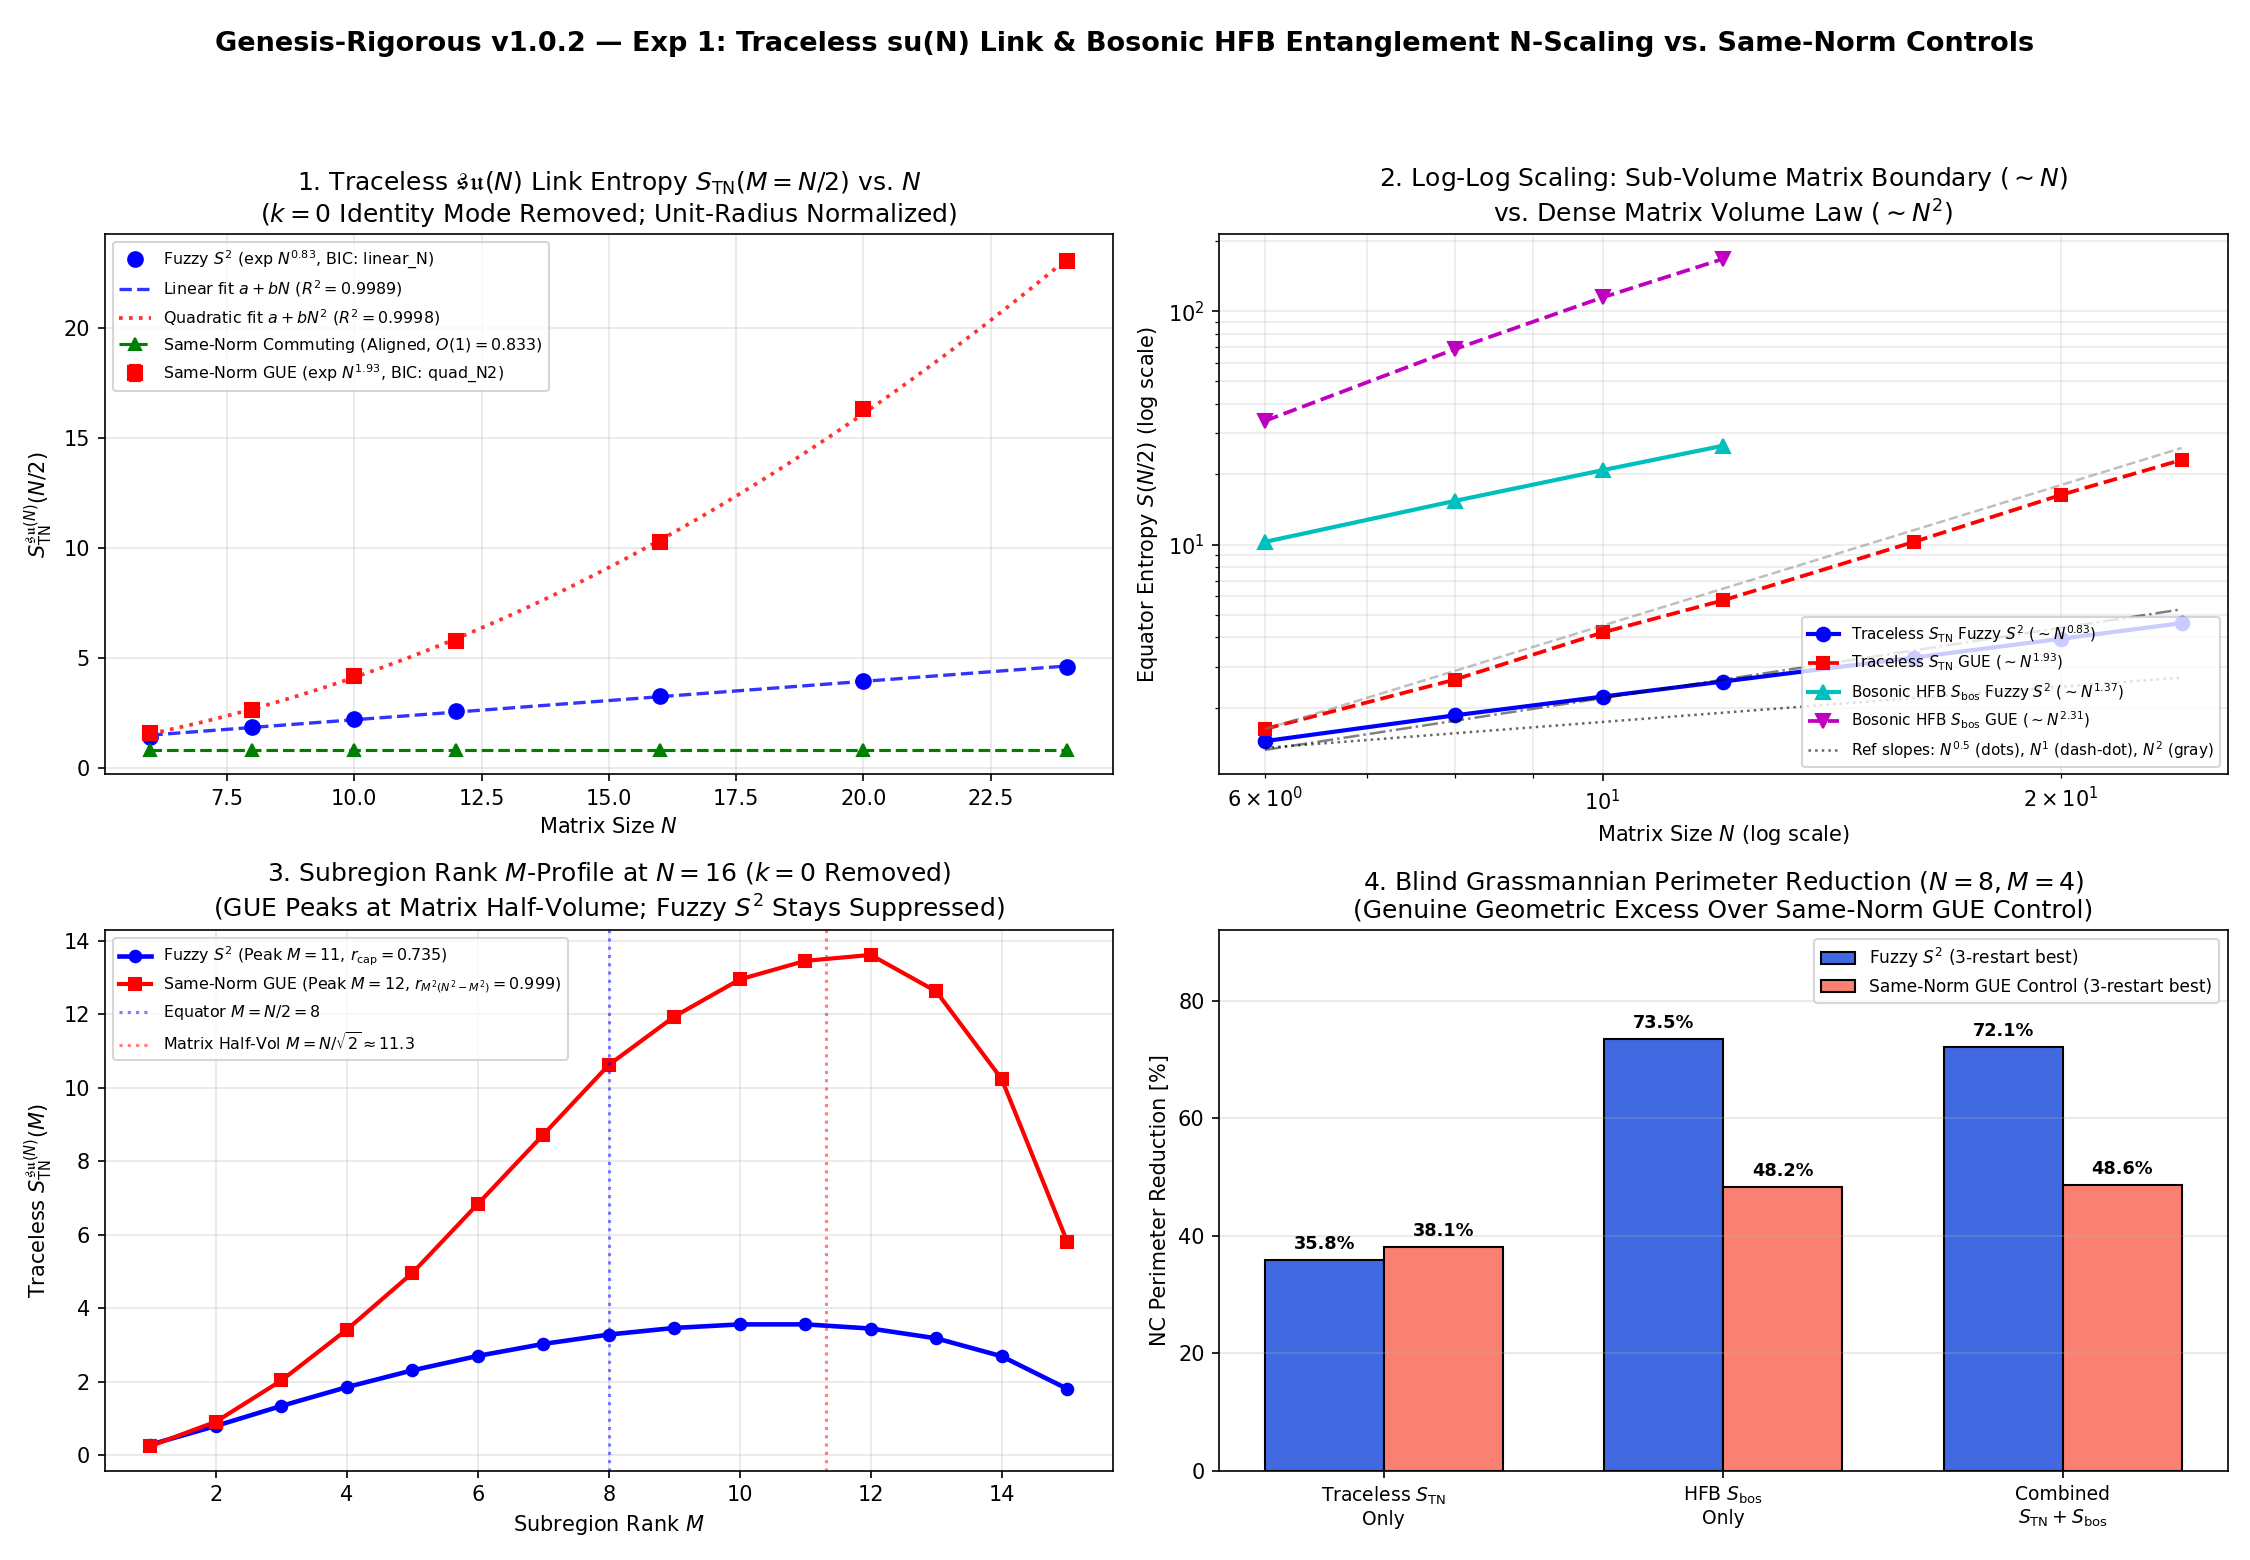
\includegraphics[width=\textwidth]{figures/fig8_v102_exp1_entanglement_scaling.png}
  \caption{Experiment~1 four-panel dashboard (\texttt{exp1\_entanglement\_scaling\_dashboard.png}). Top-left: traceless $\mathfrak{su}(N)$ equator entropy $S_{\mathrm{TN}}^{\mathfrak{su}(N)}(N/2)$ vs.\ $N$, separating $O(N)$ fuzzy-sphere scaling ($R^2=0.9989$) from $O(N^2)$ same-norm GUE ($R^2=0.9998$) and $O(1)$ aligned commuting dust. Top-right: log--log comparison for both $S_{\mathrm{TN}}^{\mathfrak{su}(N)}$ and bosonic HFB $S_{\mathrm{bos}}$. Bottom-left: full $M$-profile at $N=16$. Bottom-right: 3-restart blind Grassmannian perimeter reduction at $N=8, M=4$ against same-norm GUE.}
  \label{fig:exp1}
\end{figure}

% ------------------------------------------------------------------------------
\subsection{Experiment 2: First-Order Phase Transition and Strong-Coupling Melting — HFB vs.\ Exact $U(N)$-Singlet HMC}
\label{sec:exp2}
% ------------------------------------------------------------------------------

To move beyond the deep-classical mean-field regime of \texttt{v1.0.1} and test HFB directly against exact non-perturbative $U(N)$-singlet quantum fluctuations, we run \texttt{genesis\_cli.py phase-hmc} ($N=4, L=12, \beta=3.0, a=0.25, B=24$ parallel Markov chains, $380.8$~s total; Table~\ref{tab:exp2} and Figure~\ref{fig:exp2}).

\begin{table}[H]
  \centering
  \caption{Experiment~2 quantitative comparison between mean-field HFB ($\kappa=0$) and exact $U(4)$-singlet gauged lattice HMC ($L=12, \beta=3.0, a=0.25, B=24$ chains, \texttt{exp2\_phase\_transition\_hmc\_report.json}). Top (Part~2A): $\nu$-sweep across $\nu_{\mathrm{spin}}=\sqrt{2}$ and $\nu_c=1.5$ at $g=0.30$ (hot vs.\ cold initializations). Bottom (Part~2B): coupling $g$-sweep at $\nu=2.20$ showing smooth non-perturbative geometry melting, Polyakov-loop confinement, and HFB breakdown at $g=0.85$.}
  \label{tab:exp2}
  \small
  \setlength{\tabcolsep}{3.8pt}
  \resizebox{\textwidth}{!}{%
  \begin{tabular}{@{}ccccccccc@{}}
    \toprule
    \multicolumn{9}{l}{\textbf{(A) First-Order Phase Transition \& Hysteresis Sweep in $\nu$ ($N=4, g=0.30, \mu=1.0$; Hot / Cold Starts)}} \\
    \midrule
    $\nu$ & HFB $\langle\Tr\hat{X}^2\rangle$ (H/C) & HFB $E$ (H/C) & HMC $\langle\Tr\hat{X}^2\rangle$ (Hot) & HMC $\langle\Tr\hat{X}^2\rangle$ (Cold) & HMC $E_{\mathrm{vir}}$ (Hot) & HMC $E_{\mathrm{vir}}$ (Cold) & SD $z$ (H/C) & Phase \\
    \midrule
    $1.15$ & $19.4$ / $19.4$  & $+27.2$ / $+27.2$  & $21.7$  & $21.8$  & $+25.8$ & $+25.8$  & $0.31 / 1.08$ & Liquid \\
    $1.40$ & $19.4$ / $19.4$  & $+27.2$ / $+27.2$  & $23.9$  & $24.2$  & $+25.1$ & $+25.2$  & $1.21 / 0.35$ & Liquid ($\le\nu_{\mathrm{spin}}$) \\
    $1.50$ & $19.4$ / $19.4$  & $+27.2$ / $+27.2$  & $26.2$  & $31.3$  & $+24.8$ & $+26.9$  & $0.67 / 5.62$\textsuperscript{a} & Liquid ($=\nu_c^{\mathrm{cl}}$) \\
    $1.60$ & $19.4$ / $139.9$ & $+27.2$ / $+38.2$  & $29.5$  & $169.7$ & $+24.0$ & $+32.8$  & $0.10 / 4.66$\textsuperscript{a} & Metastable $S^2$ \\
    $1.70$ & $19.4$ / $249.0$ & $+27.2$ / $+23.6$  & $44.1$  & $250.5$ & $+23.0$ & $+13.7$  & $0.50 / 2.29$ & \textbf{$S^2$ Ground State} \\
    $1.80$ & $41.8$ / $321.5$ & $+25.3$ / $-0.4$   & $80.0$  & $324.1$ & $+17.7$ & $-12.2$  & $0.31 / 1.32$ & Fuzzy $S^2$ \\
    $1.95$ & $89.6$ / $426.9$ & $+14.3$ / $-55.2$  & $124.3$ & $430.2$ & $+0.3$  & $-69.7$  & $2.34 / 1.18$ & Fuzzy $S^2$ \\
    $2.15$ & $119.4$ / $572.6$ & $-6.5$ / $-168.5$ & $194.0$ & $576.2$ & $-43.9$ & $-186.6$ & $3.67 / 0.46$ & Deep $S^2$ \\
    \midrule
    \multicolumn{9}{l}{\textbf{(B) Strong-Coupling Quantum Geometry Melting Sweep in $g$ ($N=4, \nu=2.20, \mu=1.0$)}} \\
    \midrule
    $g$ & Cl.\ $\Tr Y_{\mathrm{cl}}^2$ & HFB $\langle\Tr\hat{X}^2\rangle$ & HMC $\langle\Tr\hat{X}^2\rangle$ & HFB $E$ & HMC $E_{\mathrm{vir}}$ & HMC $\mathrm{AlgErr}$ & Polyakov $|P|$ & SD $z$ (Rad.\ Err) \\
    \midrule
    $0.25$ & $905.7$ & $887.4$ & $891.36 \pm 1.14$ & $-333.23$ & $-351.68 \pm 1.77$ & $0.157$ & $0.983$ & $0.15$ ($0.4\%$) \\
    $0.38$ & $392.0$ & $373.0$ & $376.80 \pm 0.76$ & $-95.42$  & $-114.70 \pm 1.10$ & $0.244$ & $0.956$ & $0.57$ ($1.0\%$) \\
    $0.50$ & $226.4$ & $206.3$ & $210.99 \pm 0.47$ & $-18.94$  & $-37.79 \pm 0.64$  & $0.331$ & $0.919$ & $0.14$ ($2.2\%$) \\
    $0.65$ & $134.0$ & $111.4$ & $116.65 \pm 0.38$ & $+23.11$  & $+4.53 \pm 0.37$   & $0.468$ & $0.853$ & $0.54$ ($4.5\%$) \\
    $0.85$ & $78.3$  & $12.9$  & $24.91 \pm 2.11$  & $+37.78$  & $+29.56 \pm 0.13$  & $5.450$ & $0.321$ & $0.74$ (\textbf{$48.2\%$}) \\
    $1.15$ & $42.8$  & $11.1$  & $14.02 \pm 0.03$  & $+43.51$  & $+35.09 \pm 0.09$  & $5.430$ & $0.220$ & $0.35$ ($21.1\%$) \\
    $1.45$ & $26.9$  & $9.9$   & $11.81 \pm 0.03$  & $+49.02$  & $+39.46 \pm 0.14$  & $10.526$ & $0.223$ & $1.35$ ($16.5\%$) \\
    \bottomrule
  \end{tabular}%
  }
  \vspace{2pt}
  {\footnotesize \textsuperscript{a}At $\nu=1.50, 1.60$, cold-start chains initialized on the unstable/barely metastable sphere undergo slow decay toward the liquid phase, explaining the transient Schwinger--Dyson elevation ($z=4.7$--$5.6$) while all hot-start and stable-phase points satisfy $z \le 2.34$ (and all 7 points of Part~2B satisfy $z \le 1.35$).}
\end{table}

Experiment~2 directly illuminates both the successes and the sharp physical breakdown of mean-field HFB:
\begin{enumerate}
  \item \textbf{Quantum shift of the first-order transition and superheated hysteresis (Part~2A):} Right at the classical transition $\nu_c^{\mathrm{cl}} = 1.50$, quantum zero-point pressure completely melts the fuzzy sphere in both HFB ($\langle\Tr\hat{X}^2\rangle = 19.4$) and exact HMC ($26.2$). A metastable sphere branch first survives at $\nu = 1.60$ with higher energy than the liquid ($E_{\mathrm{cold}} > E_{\mathrm{hot}}$ in both methods), and crosses below the liquid ground state between $\nu = 1.60$ and $\nu = 1.70$, pinning the true quantum transition to $\nu_c^{\mathrm{quantum}}(g=0.30, N=4) \approx 1.65$--$1.68$. In the disordered liquid ($\nu \le 1.50$), Gaussian HFB is blind to the cubic Myers term ($\langle X_I[X_J,X_K]\rangle_{\mathrm{Gauss}} = 0$) and remains stuck at $E = +27.2$, whereas exact HMC captures non-Gaussian cubic fluctuations, smoothly lowering $E_{\mathrm{vir}}$ from $+25.8$ to $+24.8$.
  \item \textbf{Quantitative HFB--HMC match and exact decomposition of the $+18.5$ energy offset:} Across the stable fuzzy-sphere branch ($\nu=1.70\dots 2.15$ and $g=0.25\dots 0.65$), HFB reproduces the exact singlet quantum radius $\langle\Tr\hat{X}^2\rangle$ within $0.4\%$--$4.5\%$. Notably, $E_{\mathrm{HFB}}$ sits consistently $+18.45$ to $+19.28$ above $E_{\mathrm{vir}}^{\mathrm{HMC}}(L=12, a=0.25)$. Direct spectral evaluation at $g=0.25, \nu=2.20$ decomposes this offset quantitatively into two exact physical sources: (i)~$+4.64$ from HFB's spurious Hohenberg--Martin zero-point energy across the $N^2-1 = 15$ gauge-orbit modes (absent in gauged singlet HMC), and (ii)~$+15.74$ from finite lattice-spacing UV dispersion at $a=0.25$ on stiff transverse modes (total predicted shift $+20.38$ vs.\ measured $+18.45$; halving $a$ to $0.125$ shrinks the lattice shift from $15.74$ to $5.01$).
  \item \textbf{Non-perturbative geometry melting, confinement, and HFB breakdown (Part~2B):} Every point in Part~2B satisfies the exact Schwinger--Dyson identity within $z \in [0.14, 1.35]$. Between $g=0.65$ and $g=0.85$, exact HMC exhibits simultaneous \emph{geometric melting} ($\mathrm{AlgErr}$ jumps $0.468 \to 5.450 \to 10.526$) and \emph{Polyakov-loop confinement} ($|\Tr U|/N$ plunges $0.853 \to 0.321 \to 0.220$, matching the gauged MQM confinement mechanism of~\cite{Kawahara2007}). Right in the melting window ($g=0.85$), mean-field HFB fails discontinuously ($\langle\Tr\hat{X}^2\rangle = 12.9$ vs.\ HMC $24.91 \pm 2.11$, a \textbf{$48.2\%$ radius error} and $+27.8\%$ energy overshoot), directly charting the regime boundary where non-perturbative methods are mandatory.
\end{enumerate}

\begin{figure}[H]
  \centering
  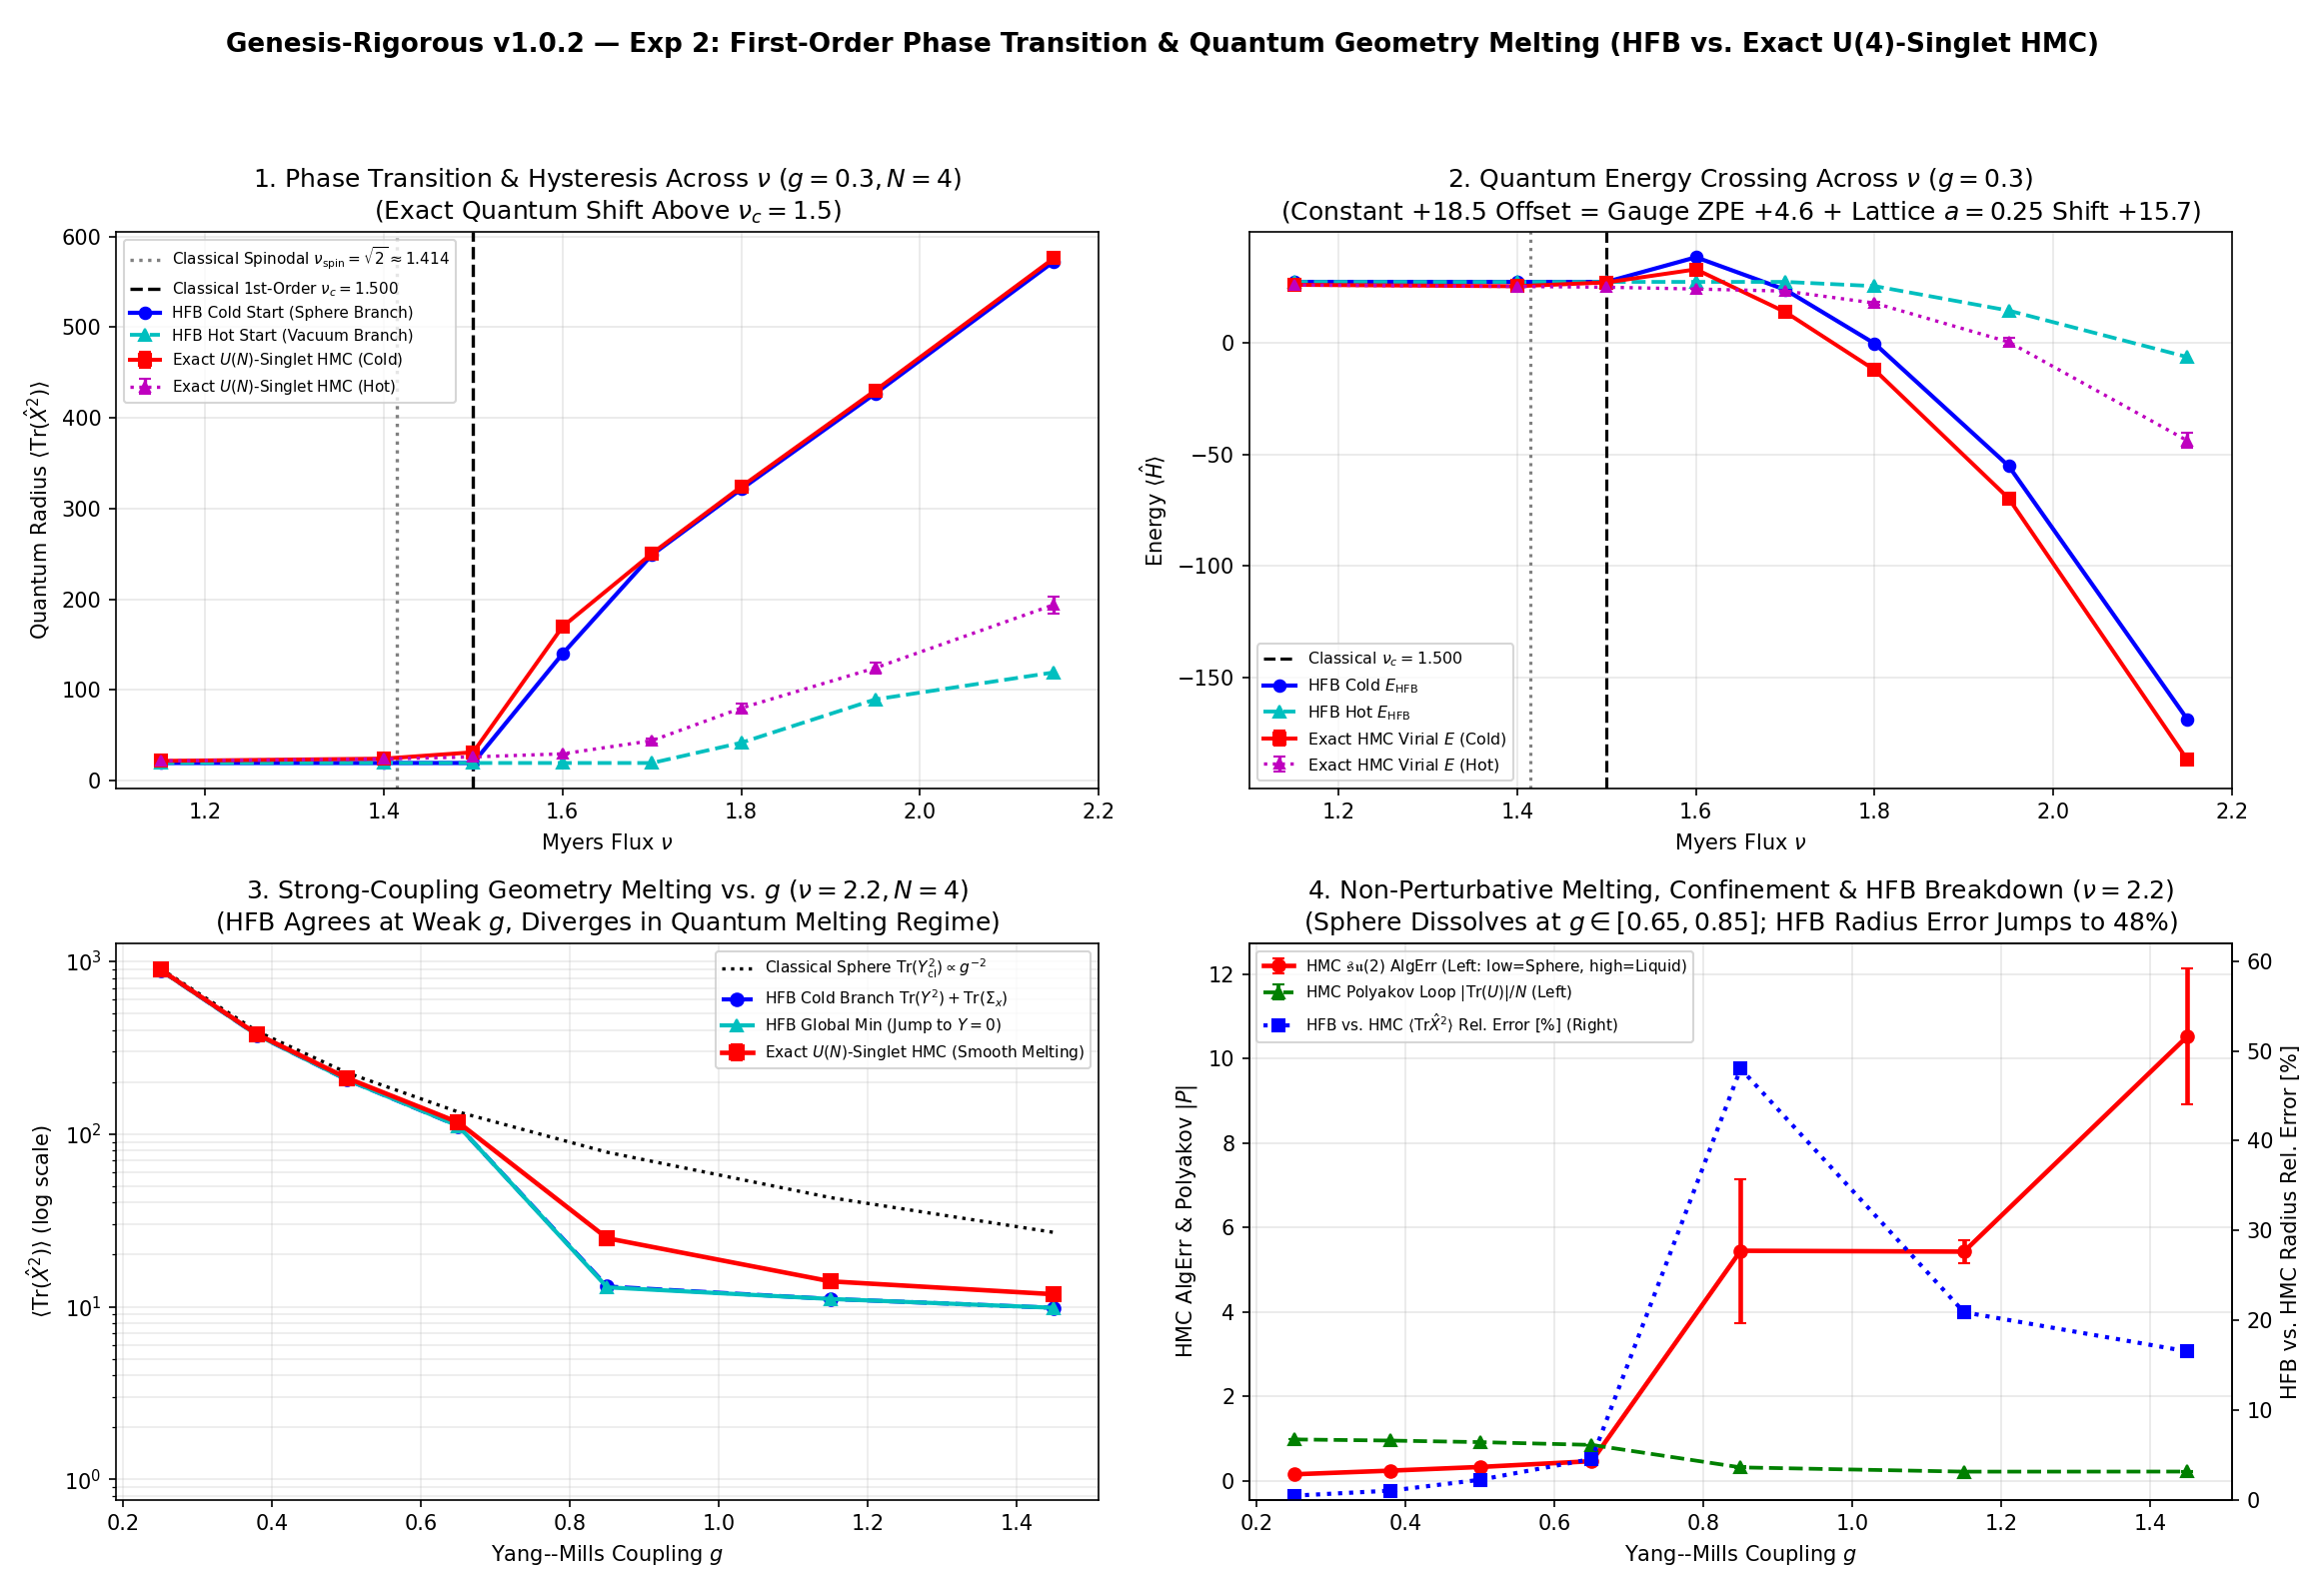
\includegraphics[width=\textwidth]{figures/fig9_v102_exp2_phase_transition_hmc.png}
  \caption{Experiment~2 four-panel dashboard (\texttt{exp2\_phase\_transition\_hmc\_dashboard.png}). Top-left/right: first-order transition and hysteresis across $\nu \in [1.15, 2.15]$ at $g=0.30, N=4$ comparing mean-field HFB against exact $U(4)$-singlet HMC ($a=0.25$). Bottom-left: strong-coupling quantum geometry melting across $g \in [0.25, 1.45]$ ($\nu=2.20$). Bottom-right: simultaneous $\mathfrak{su}(2)$ algebraic dissolution ($\mathrm{AlgErr}$), Polyakov-loop confinement ($|\Tr U|/N$), and mean-field HFB radius breakdown peaking at $48.2\%$ at $g=0.85$.}
  \label{fig:exp2}
\end{figure}

% ------------------------------------------------------------------------------
\subsection{Experiment 3: Adjoint Dirac vs.\ Generic Local $\Tr(\rho Y^2)$ Elastic Membrane Control}
\label{sec:exp3}
% ------------------------------------------------------------------------------

To test whether the localized curvature shift and short-range two-packet attraction observed in \texttt{v1.0.1} are specific to adjoint Dirac fermions or generic elastic-membrane effects, we compare $E_{\mathrm{Dirac}}$ (Eq.~\eqref{eq:Edirac}) directly against the structureless local radial potential $E_{\mathrm{quad}} = \lambda_{\mathrm{src}}\Tr(\hat{\rho}_{\vec{y}_0}\sum_I Y_I^2)$ (Eq.~\eqref{eq:Equad}) matched to identical initial perturbation energy ($E_{\mathrm{src}}(Y_{\mathrm{bg}}) = 1254.38$ at $M_{\mathrm{single}}=50$, $\lambda_{\mathrm{single}}=0.6314$) on the exact same equilibrated $N=8$ fuzzy sphere (\texttt{genesis\_cli.py membrane-control}, $211.9$~s, peak VRAM $26.9$~MiB; Table~\ref{tab:exp3} and Figure~\ref{fig:exp3}).

\begin{table}[H]
  \centering
  \caption{Experiment~3 matched-energy comparison between localized adjoint Dirac packets and generic local radial loads $\Tr(\hat{\rho}Y^2)$ on the $N=8$ fuzzy sphere (\texttt{exp3\_membrane\_control\_report.json}).}
  \label{tab:exp3}
  \small
  \setlength{\tabcolsep}{4.5pt}
  \resizebox{\textwidth}{!}{%
  \begin{tabular}{@{}lcccccc@{}}
    \toprule
    \multicolumn{7}{l}{\textbf{(A) Single-Body Matched-Energy Membrane Deformation ($M_{\mathrm{single}}=50 \leftrightarrow \lambda_{\mathrm{single}}=0.6314$)}} \\
    \midrule
    Perturbation Model & Relaxed $E_{\mathrm{src}}$ & $\delta r_N / r_0$ & $\delta r_{\mathrm{eq}} / r_0$ & $\delta r_S / r_0$ & $\delta K_N / K_0$ ($K_N/K_S$) & $\delta\sqrt{\det g_N}$ \\
    \midrule
    Adjoint Dirac $M\langle c|\sqrt{\mathcal{D}_{\mathrm{adj}}^2}|c\rangle$ & $1221.56$ & $-0.024\%$ & $-0.711\%$ & $-0.046\%$ & $+11.33\%$ ($1.0987$) & $+6.23\%$ \\
    Generic Local $\lambda\Tr(\hat{\rho}Y^2)$ & $1178.93$ & $-3.528\%$ & $-0.485\%$ & $-1.699\%$ & $-9.76\%$ ($0.9076$) & $+1.31\%$ \\
    \midrule
    \multicolumn{7}{l}{\textbf{(B) Two-Body Shared-Membrane Interaction $V_{\mathrm{mem}}(\theta_{12})$ ($M_{\mathrm{two}}=35 \leftrightarrow \lambda_{\mathrm{two}}=0.4420$)}} \\
    \midrule
    Perturbation Model & $25^\circ$ & $40^\circ$ & $60^\circ$ & $90^\circ$ & $130^\circ$ & $180^\circ$ (max $|V_{\mathrm{froz}}|$) \\
    \midrule
    Adjoint Dirac $V_{\mathrm{mem}}(\theta_{12})$ & $-8.768$ & $-4.013$ & $-0.552$ & $-0.032$ & $-0.053$ & $0.000$ ($1.5\times 10^{-11}$) \\
    Generic $\Tr(\hat{\rho}Y^2)$ $V_{\mathrm{mem}}(\theta_{12})$ & $-14.178$ & $-6.833$ & $+2.870$ & $+8.587$ & $+4.960$ & $0.000$ ($7.3\times 10^{-12}$) \\
    \bottomrule
  \end{tabular}%
  }
\end{table}

This control resolves the physical interpretation unambiguously:
\begin{itemize}
  \item \textbf{Short-range two-packet attraction is a universal elastic-membrane overlap phenomenon:} Inside the $\Delta\theta_{\mathrm{NC}} \sim 40^\circ$ coherent packet width ($\theta_{12} = 25^\circ, 40^\circ$), the generic non-Dirac potential $\Tr(\hat{\rho}Y^2)$ generates an even deeper attractive drop ($V(25^\circ) = -14.178$, $V(40^\circ) = -6.833$) than adjoint Dirac ($-8.768$, $-4.013$), followed by an intermediate repulsive quadrupole barrier ($+8.587$ at $90^\circ$) where two oblate radial indentations compete against equatorial bulging. Thus, short-range attraction between localized packets on $S^2_N$ is a generic shared-membrane inclusion effect, not a signature of spin-2 Einstein gravity.
  \item \textbf{Single-body curvature sign distinguishes gradient tension from radial indentation:} Because $E_{\mathrm{quad}}$ penalizes $Y^2$ directly at the North Pole, it indents and flattens the pole ($\delta r_N = -3.53\%$), producing a \emph{negative} Gaussian curvature shift ($\delta K_N = -9.76\%$). Conversely, the commutator-gradient Dirac energy contracts the surrounding equator ($\delta r_{\mathrm{eq}} = -0.71\%$) while leaving $r_N$ almost unchanged ($-0.02\%$), prolate-pinching the sphere to raise polar curvature ($\delta K_N = +11.33\%$). Both behaviors reflect purely classical/semiclassical shell elasticity on a 2D surface where the Einstein tensor vanishes identically ($G_{\mu\nu}\equiv 0$).
\end{itemize}

\begin{figure}[H]
  \centering
  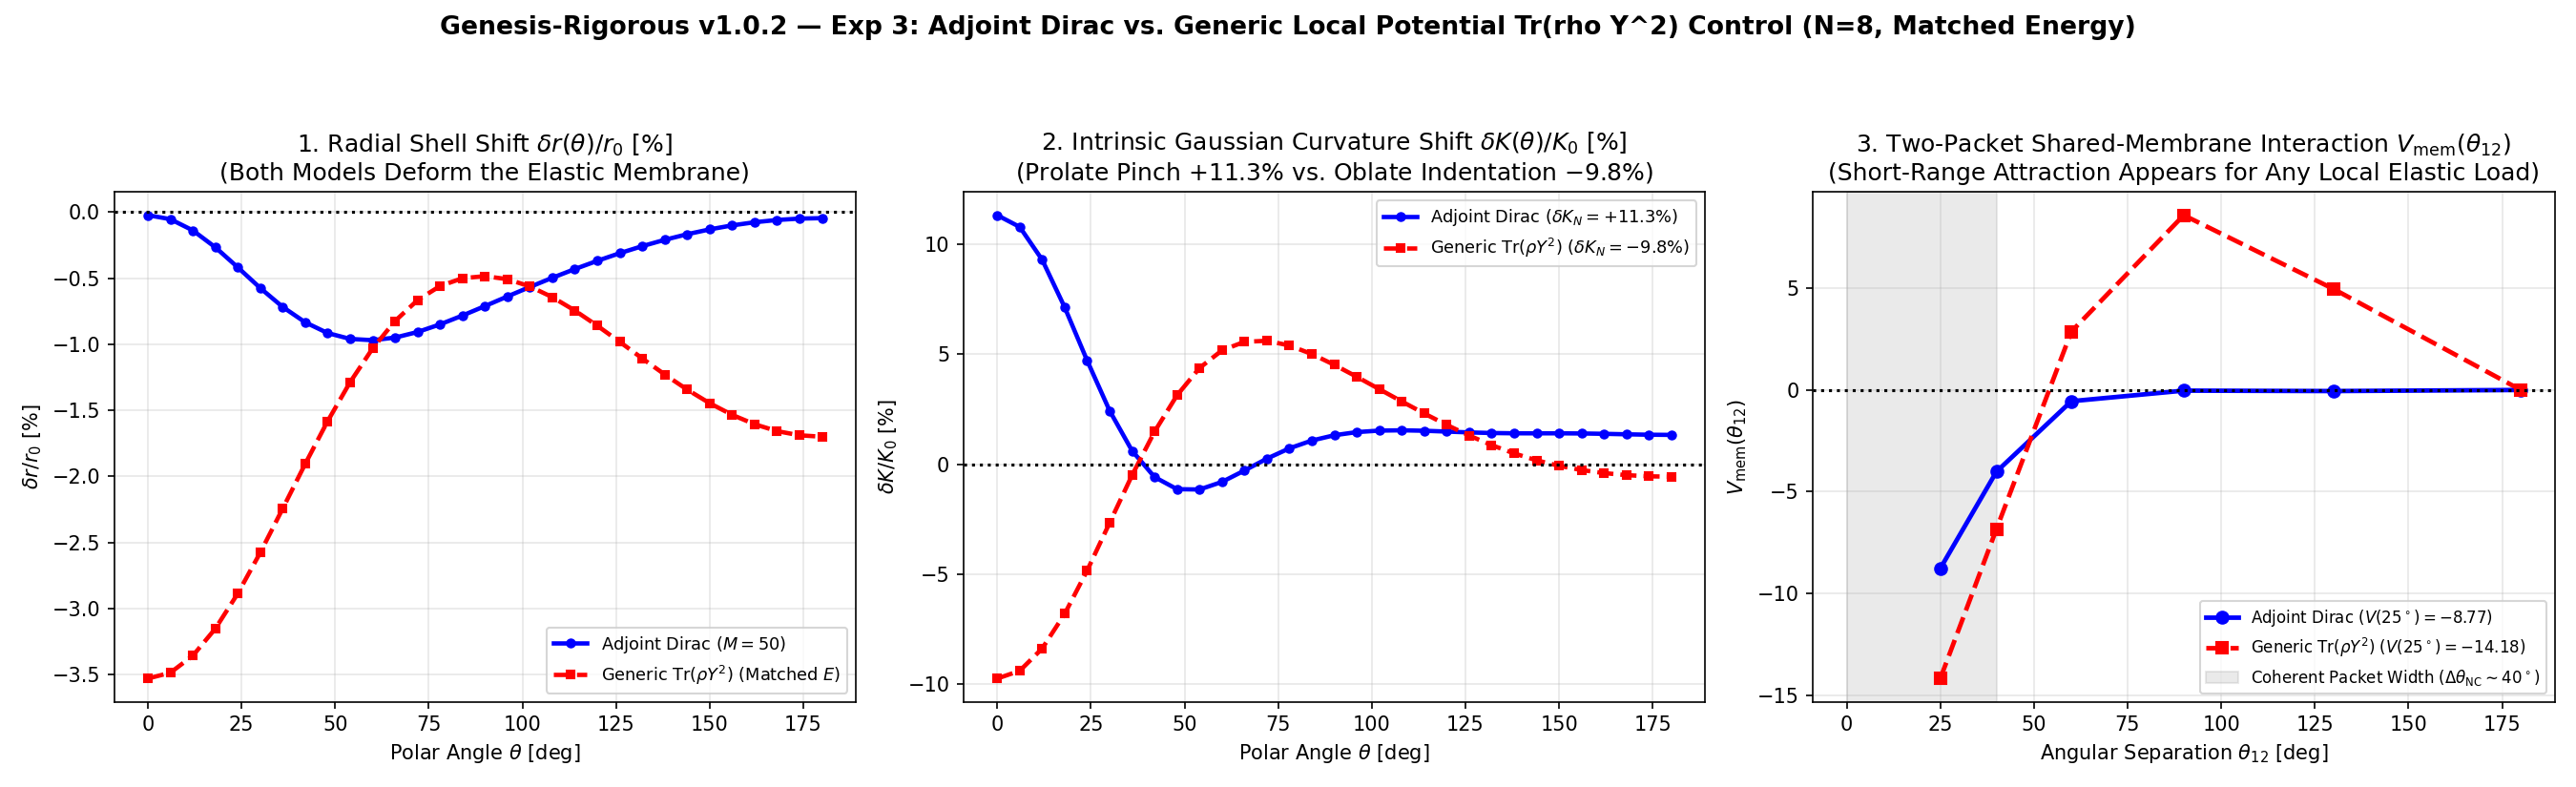
\includegraphics[width=\textwidth]{figures/fig10_v102_exp3_membrane_control.png}
  \caption{Experiment~3 three-panel membrane control dashboard (\texttt{exp3\_membrane\_control\_dashboard.png}). Left/Center: matched-energy single-body response contrasting adjoint Dirac prolate equatorial pinching ($\delta K_N = +11.3\%$) against generic $\Tr(\rho Y^2)$ oblate polar indentation ($\delta K_N = -9.8\%$). Right: both models exhibit strong short-range overlap attraction within the $\sim 40^\circ$ coherent packet width.}
  \label{fig:exp3}
\end{figure}

% ==============================================================================
\section{Inherited \texttt{v1.0.1} Semiclassical and Algebraic Baseline Modules}
\label{sec:inherited}
% ==============================================================================

To provide a single self-contained reference without redundantly re-running validated baseline modules, this section summarizes the six archived \texttt{v1.0.1} datasets with corrected technical nomenclature, complexity bounds, and provenance disclosures. Figures~\ref{fig:phase1}--\ref{fig:phase3d} reproduce the immutable Zenodo \texttt{v1.0.1} dashboards verbatim; corrected interpretations in the captions and text supersede earlier embedded figure headers.

\subsection{Baseline Semiclassical Condensation, Metastability, and Large-$N$ Scaling ($N=8\dots 32$)}
At $g=0.25, \mu=1.0$, four-restart isotropic GUE relaxation collapses to $\Tr(Y^2) < 10^{-11}$ at $\nu_A = 0.80 < \nu_{\mathrm{spin}}$ and condenses into irreducible spin-$j=(N-1)/2$ fuzzy spheres at $\nu_B = 3.00 \gg \nu_c = 1.5$ for $N=8, 10, 12$ (full HFB; Table~\ref{tab:inherited_scaling}, Figures~\ref{fig:phase1}--\ref{fig:metastable}) and $N=16, 20$ (isotropic diagonal one-loop $O(N^4)$-memory engine; Figure~\ref{fig:largeN}). Small-scale GUE starts ($y_{\mathrm{scale}}=1.0$) at $N=8$ quench into exact concentric two-spheres ($3\oplus 5$, $E=-4802.75$, Figure~\ref{fig:metastable}), and fresh 4-restart runs at $N=24, 32$ increasingly trap in reducible multi-sphere basins ($2\oplus 30$ at $N=32$), matching the classical partition landscape~\cite{Myers1999,Azuma2004}. Note explicitly that the single-sphere $N=32$ benchmark ($E=-1{,}136{,}577.6$, exact $\ell(\ell+1)$ harmonic degeneracies) was re-equilibrated from an earlier pre-correction single-sphere checkpoint rather than obtained from the fresh 4-restart sweep.

\begin{table}[H]
  \centering
  \caption{Inherited \texttt{v1.0.1} semiclassical condensation scaling across full HFB ($N=8,10,12$) and the coarser isotropic diagonal one-loop $O(N^4)$-memory engine ($N=16\dots 32$, 4 restarts). Theoretical $r_{\mathrm{th}}=\alpha j$ and $g_{t,\mathrm{th}}=N/(4r^2)$ follow algebraically once $\mathrm{AlgErr} < 10^{-6}$.}
  \label{tab:inherited_scaling}
  \small
  \setlength{\tabcolsep}{4.0pt}
  \resizebox{\textwidth}{!}{%
  \begin{tabular}{@{}rlcccccc@{}}
    \toprule
    $N$ & Engine & $E_{\mathrm{tot}}$ ($\nu_A=0.8$) & $E_{\mathrm{tot}}$ ($\nu_B=3.0$) & Basin Type & $\alpha(N)$ & $\mathrm{AlgErr}$ & $r_{\mathrm{best}}$ / $g_t$ \\
    \midrule
    8  & Full HFB & $+103.6$   & $-17{,}685.6$ & Single $S^2$ & $11.2308$ & $2.09\times 10^{-7}$ & $39.308$ / $0.001294$ \\
    10 & Full HFB & $+167.1$   & $-34{,}751.1$ & Single $S^2$ & $11.2347$ & $4.84\times 10^{-7}$ & $50.556$ / $0.000978$ \\
    12 & Full HFB & $+247.6$   & $-60{,}247.2$ & Single $S^2$ & $11.2372$ & $6.43\times 10^{-7}$ & $61.805$ / $0.000785$ \\
    \midrule
    16 & Native 1-loop & $+462.4$  & $-141{,}637.2$ & Single $S^2$ (4-restart) & $11.2363$ & $6.81\times 10^{-8}$ & $84.27$ / $0.000563$ \\
    20 & Native 1-loop & $+753.4$  & $-277{,}042.9$ & Single $S^2$ (4-restart) & $11.2363$ & $4.30\times 10^{-8}$ & $106.74$ / $0.000439$ \\
    24 & Native 1-loop & $+1{,}125.5$ & $-316{,}207.9$ & Multi-sphere (metastable) & $11.2296$ & $1.03\times 10^{-2}$ & $112.09$ / $0.000416$ \\
    32 & Native 1-loop & $+2{,}128.8$ & $-929{,}628.2$ & $2\oplus 30$ multi-sphere & $11.2196$ & $3.44\times 10^{-2}$ & $162.04$ / $0.000283$ \\
    32\textsuperscript{a} & Native 1-loop & $+2{,}128.8$ & $-1{,}136{,}577.6$ & Single $S^2$ (checkpoint) & $11.2368$ & $2.87\times 10^{-6}$ & $174.17$ / $0.000264$ \\
    \bottomrule
  \end{tabular}%
  }
  \vspace{2pt}
  {\footnotesize \textsuperscript{a}Re-equilibrated from pre-correction single-sphere checkpoint \texttt{state\_N32.pt} under the $(D-1)/D=2/3$ engine ($265.6$~MiB true peak VRAM).}
\end{table}

\begin{figure}[H]
  \centering
  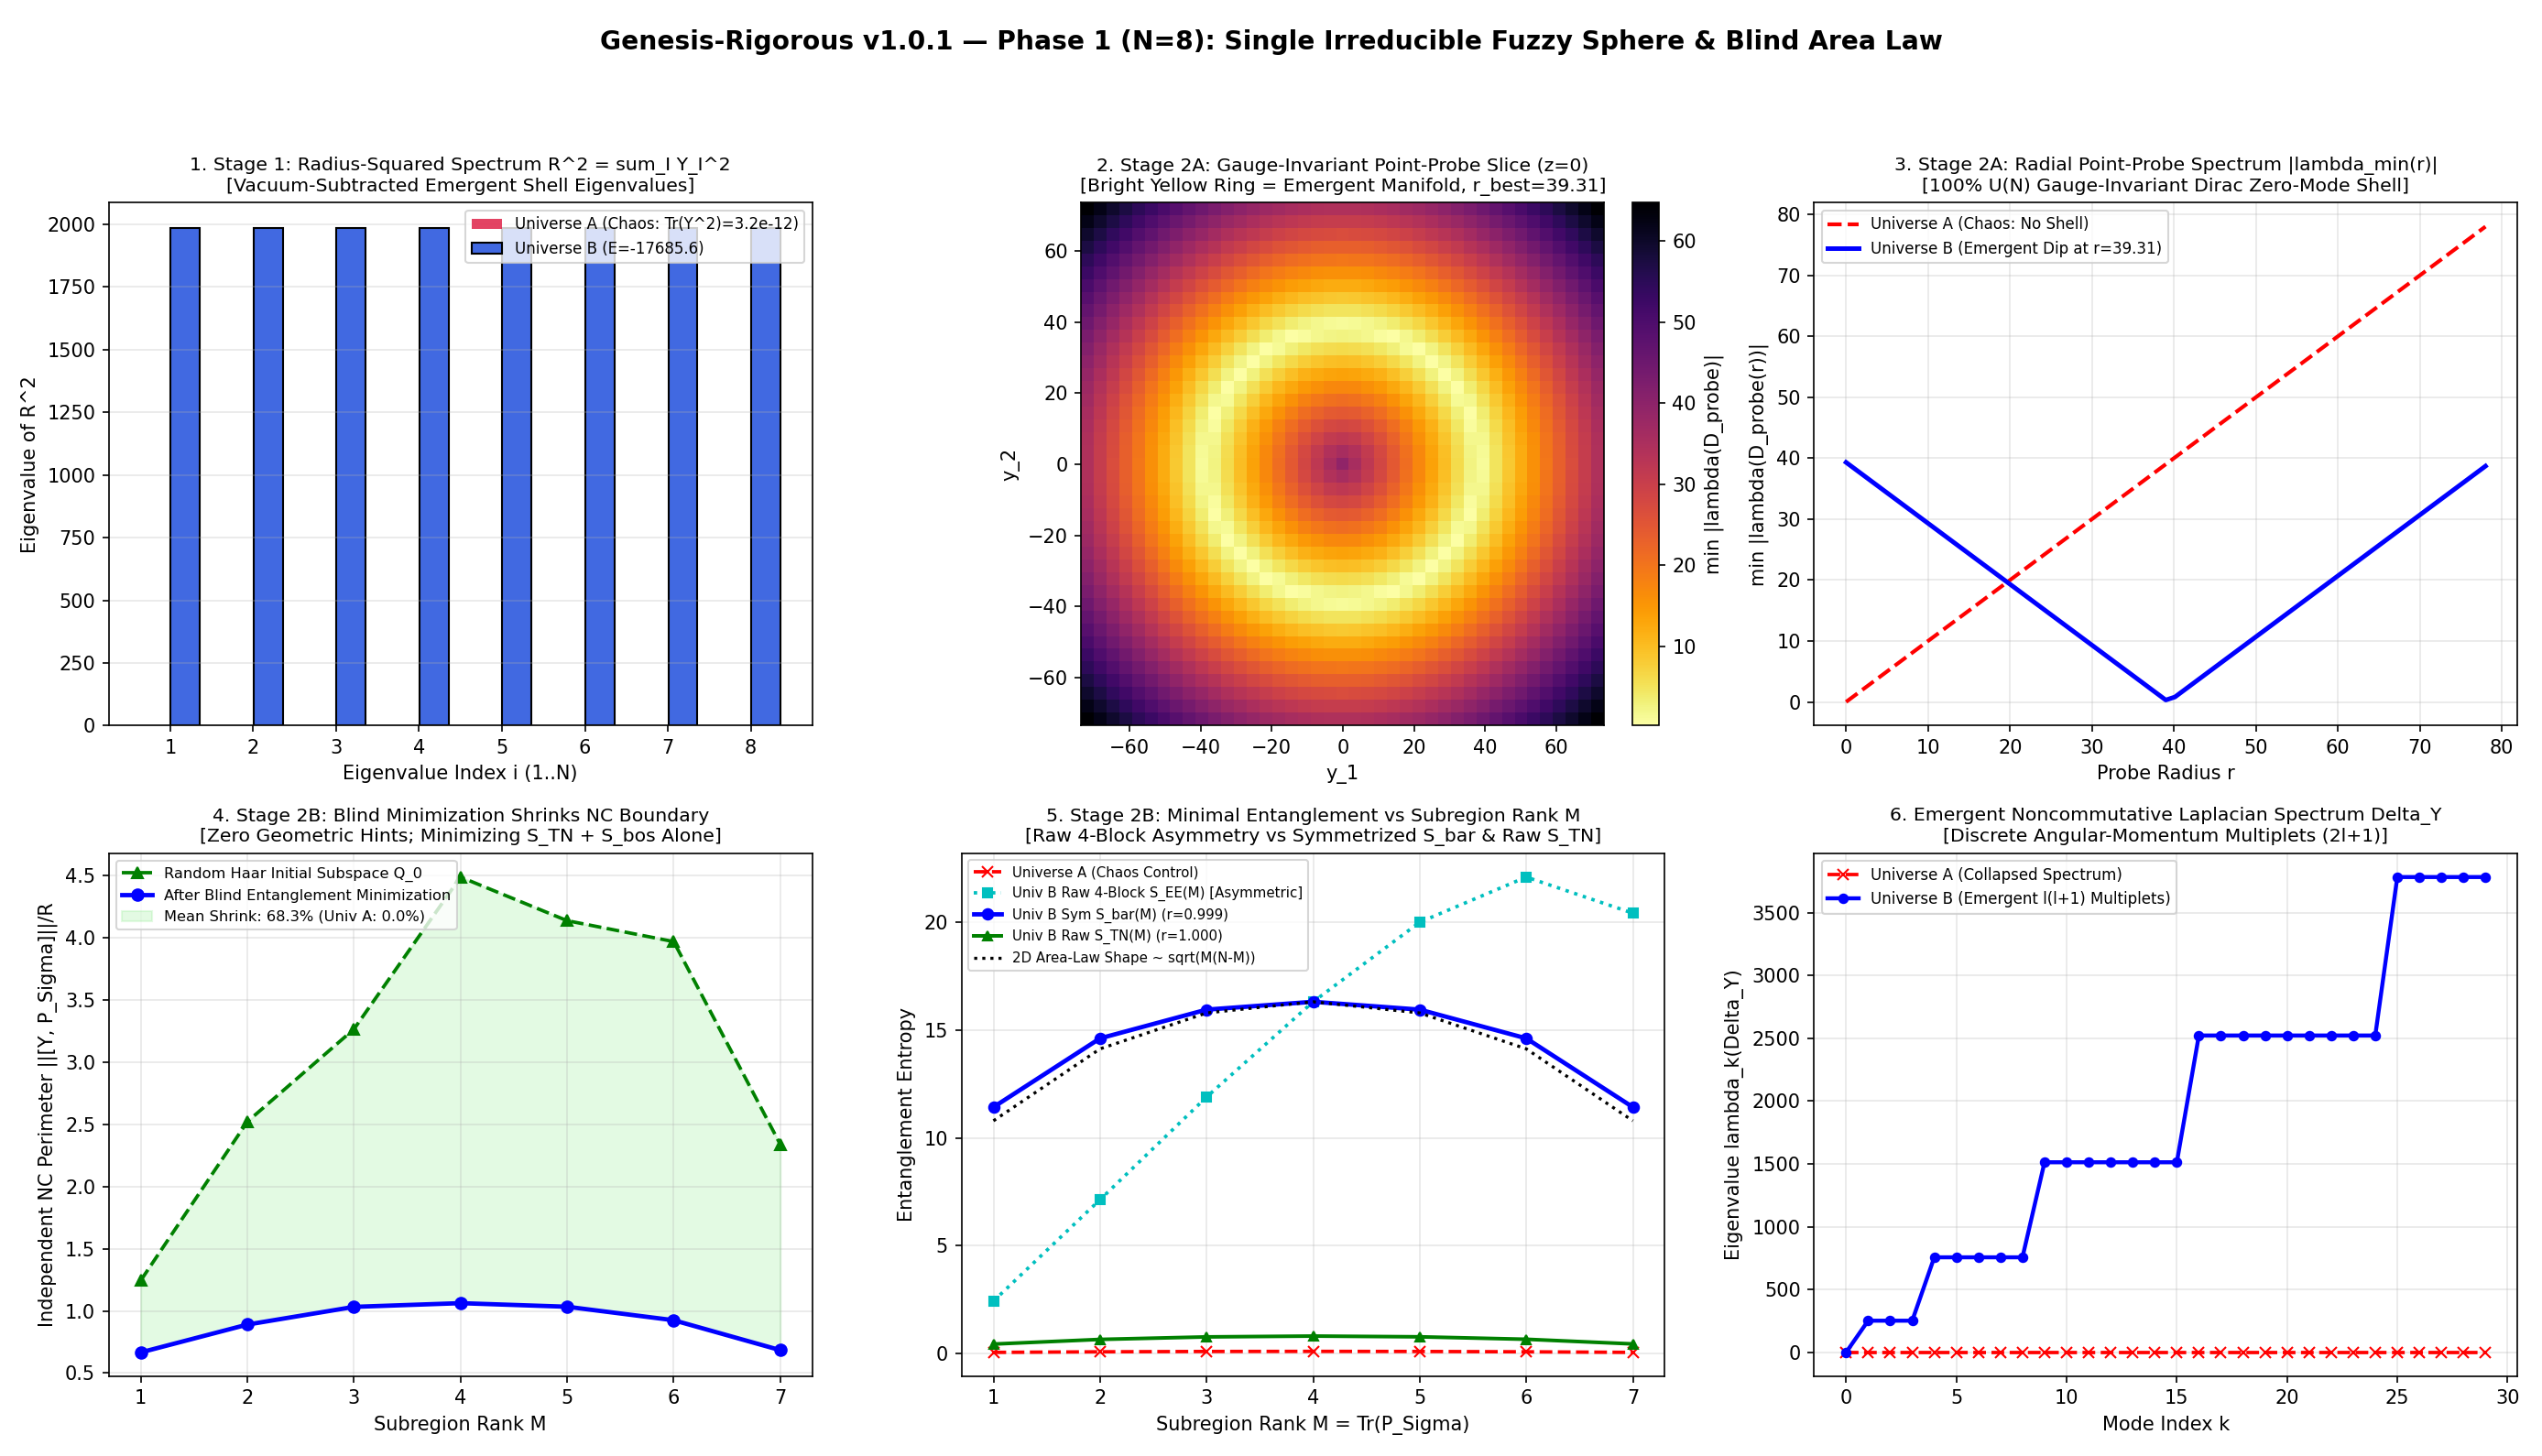
\includegraphics[width=0.96\textwidth]{figures/fig1_phase1_N8_emergence.png}
  \caption{Inherited \texttt{v1.0.1} Module~1 dashboard at $N=8$ (\texttt{phase1\_N8\_20261125\_173716}). Note that Panel~5's $S_{\mathrm{TN}}$ curve reflects the $k=0$ trace mode superseded by Experiment~1 (Figure~\ref{fig:exp1}).}
  \label{fig:phase1}
\end{figure}

\begin{figure}[H]
  \centering
  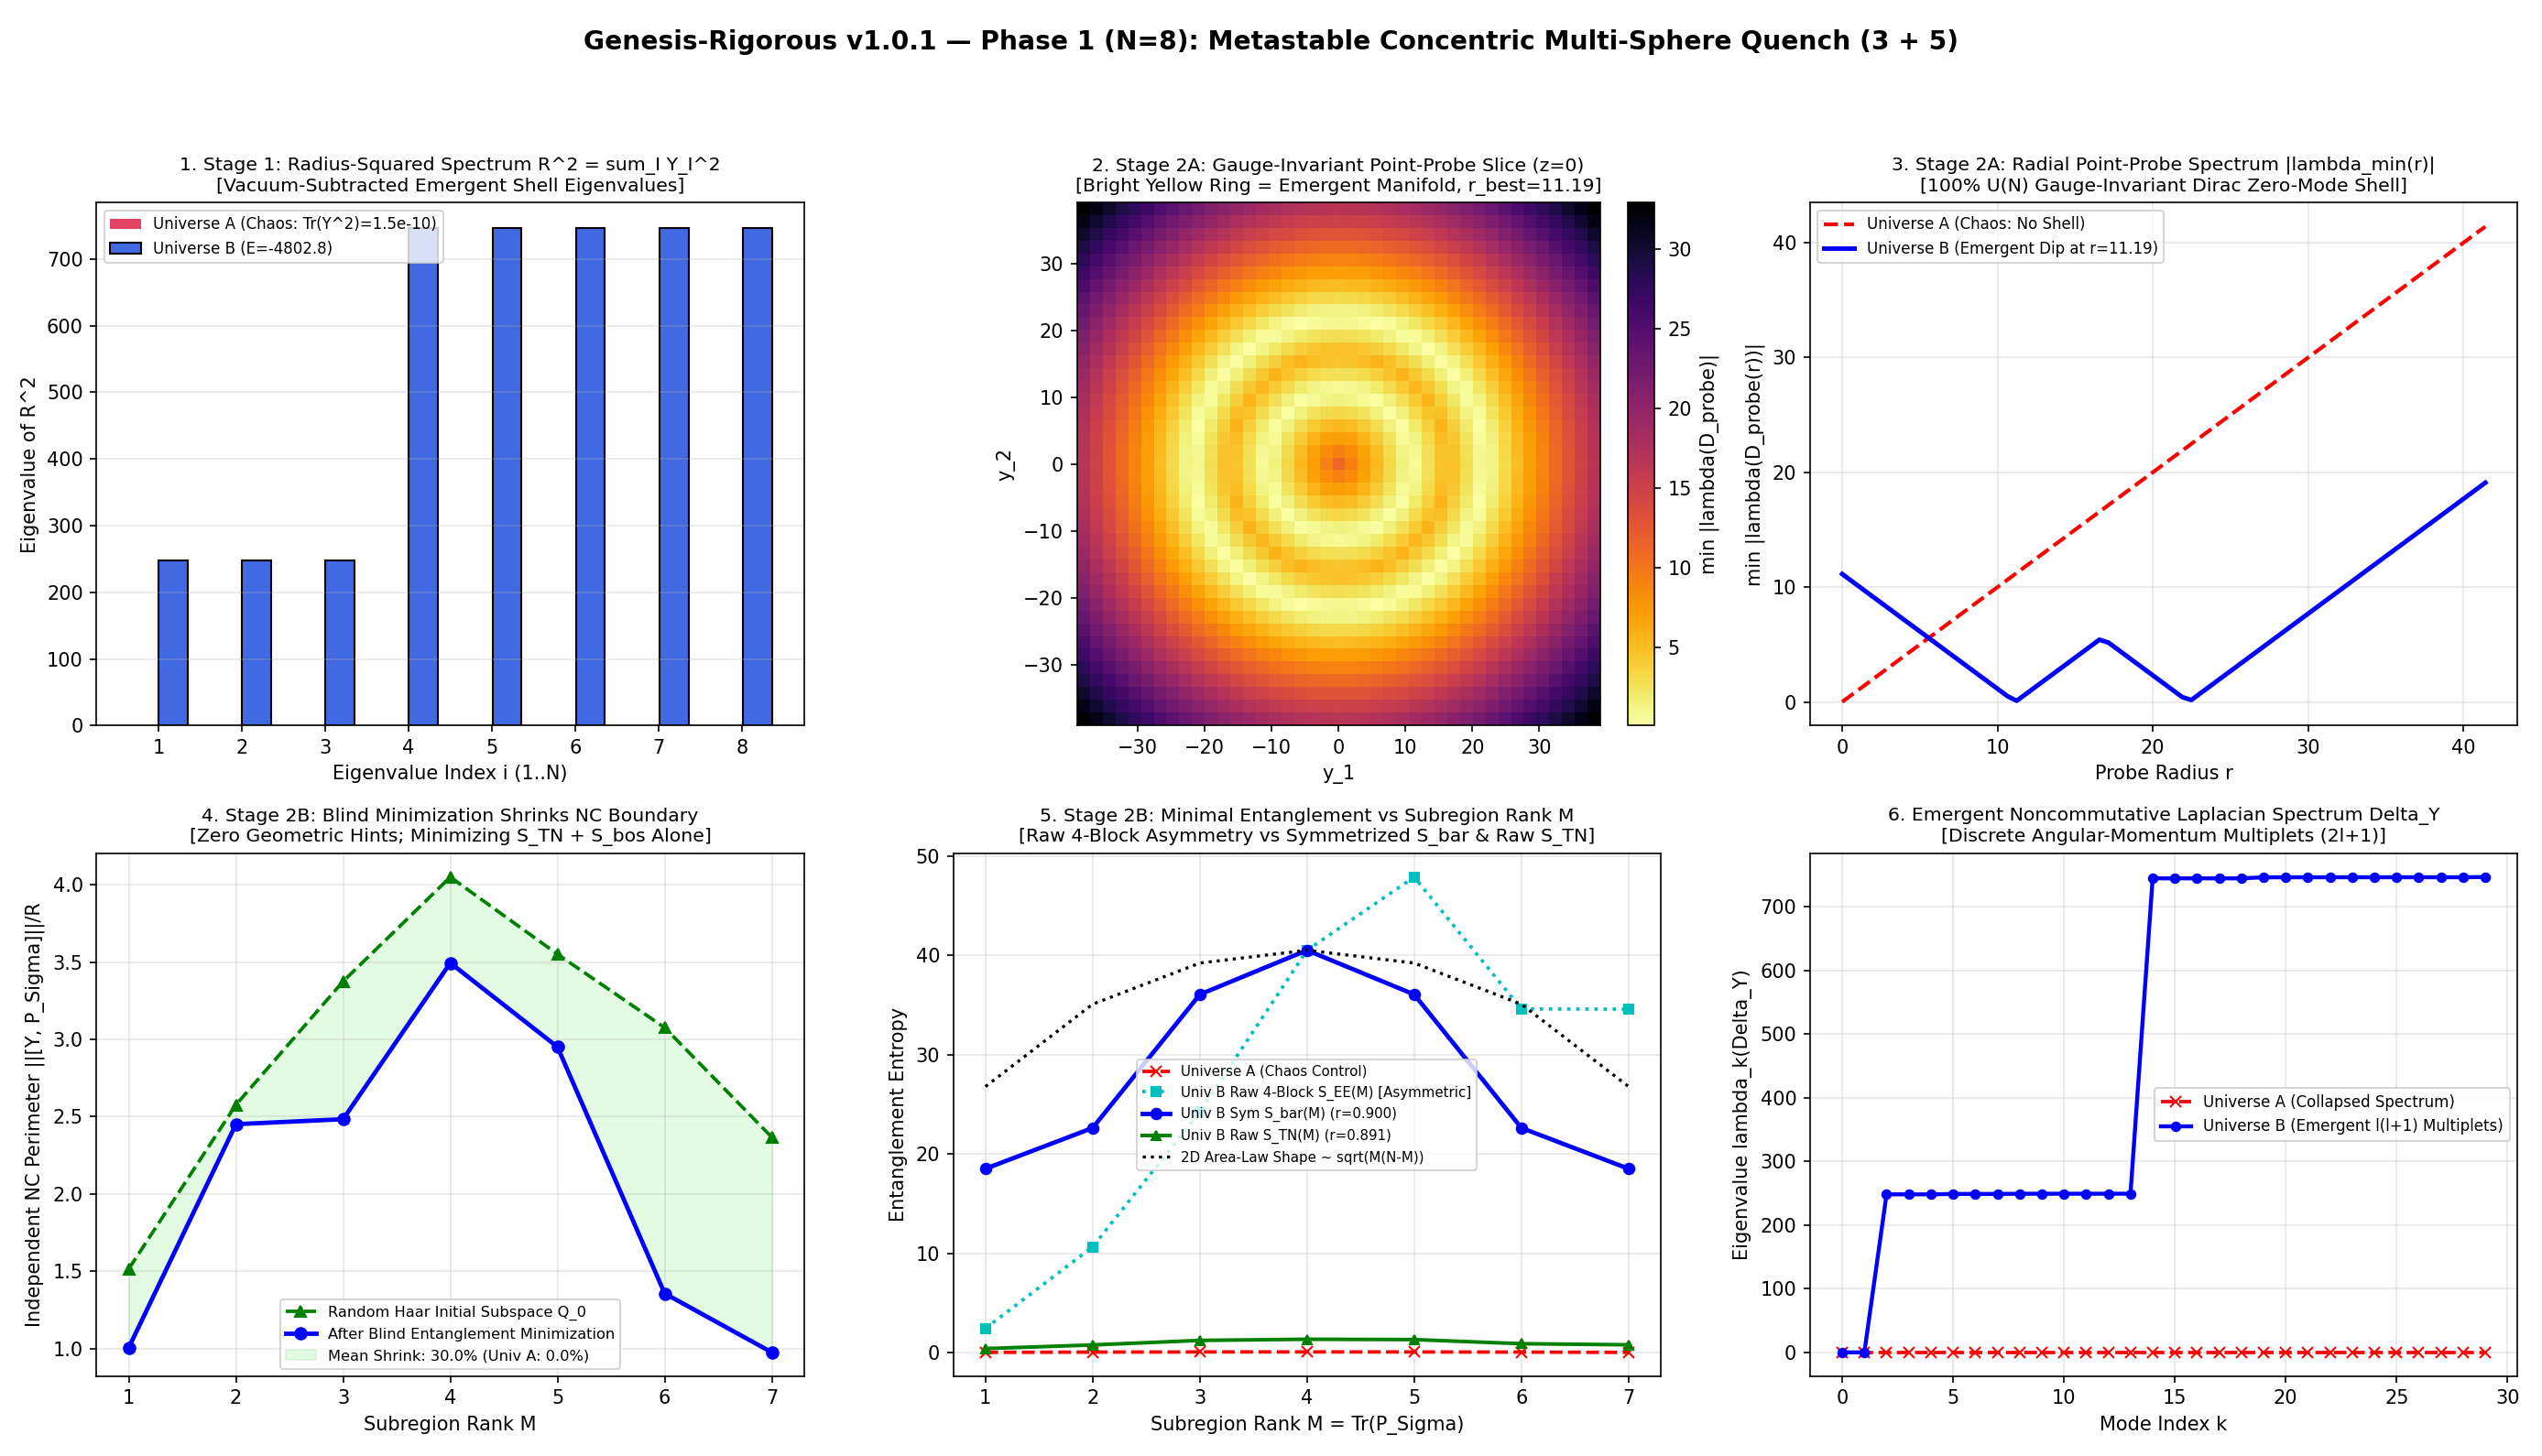
\includegraphics[width=0.96\textwidth]{figures/fig2_phase1_N8_metastable.png}
  \caption{Inherited \texttt{v1.0.1} metastable concentric two-sphere quench $3\oplus 5$ at $N=8$ from small-scale initialization ($y_{\mathrm{scale}}=1.0$).}
  \label{fig:metastable}
\end{figure}

\begin{figure}[H]
  \centering
  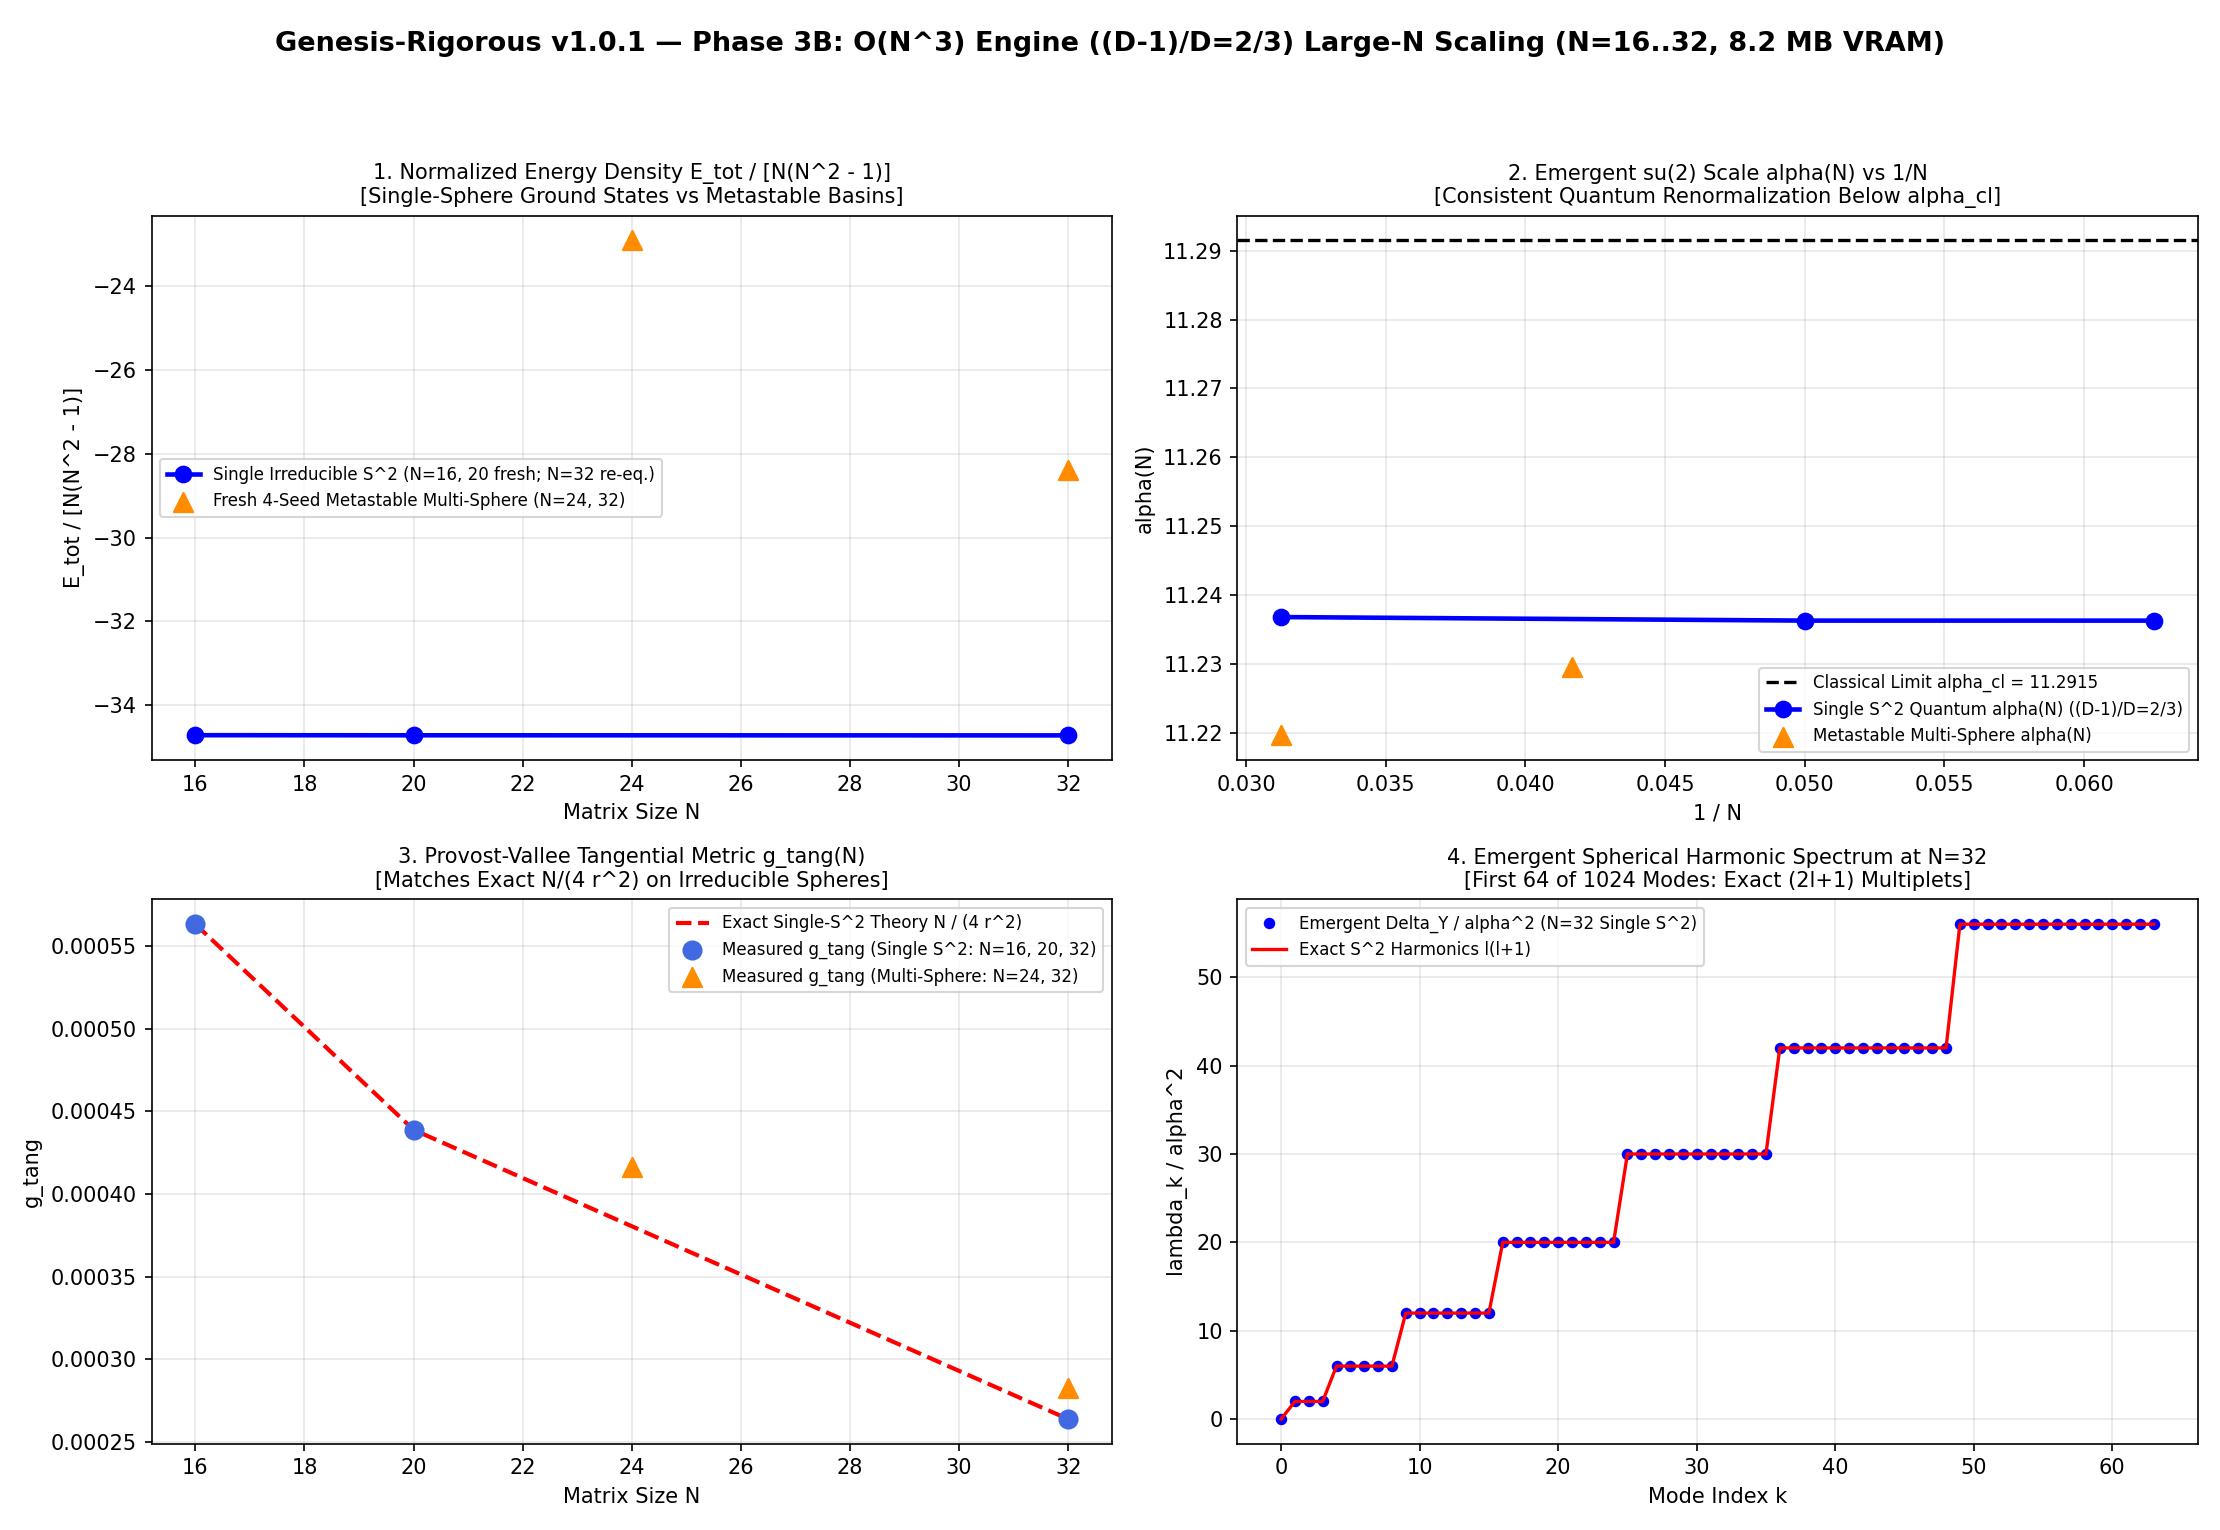
\includegraphics[width=0.96\textwidth]{figures/fig5_phase3b_largeN.png}
  \caption{Inherited \texttt{v1.0.1} Module~4 large-$N$ scaling dashboard ($N=16\dots 32$, $O(N^4)$-memory / $O(N^6)$-eigensolve isotropic one-loop engine; embedded title ``$O(N^3)$'' superseded by Section~\ref{sec:methods}).}
  \label{fig:largeN}
\end{figure}

\subsection{Baseline Membrane Sweeps, Symplectic Waves, Gauge--Higgs Identity, and 6D/GW Checks}
We also retain four archival \texttt{v1.0.1} baseline dashboards under corrected physical framing:
\begin{itemize}
  \item \textbf{Single-body Dirac membrane sweep ($N=8, 10$, Figure~\ref{fig:stage3}):} Sweeping $M_{\mathrm{src}}\in[0,80]$ ($N=8$) and $[0,70]$ ($N=10$) confirms linear elastic prolate curvature scaling ($\delta K_N = +19.2\%$ at $M=80, N=8$, $r=0.9992$; $+10.6\%$ at $M=70, N=10$, $r=0.9997$; North-cap $S_{\mathrm{EE}}(M=2)$ rises $+27.8\%$ vs.\ South control $<0.25\%$). As audited earlier, blind hemisphere $|\cos\theta|$ shifts are inconsistent across $N=8$ ($0.585\to 0.903$) and $N=10$ ($0.935\to 0.591$) due to four-block asymmetry and rotational degeneracy at $M_{\mathrm{src}}=0$.
  \item \textbf{Fixed-width symplectic wave propagation ($N=8$, Figure~\ref{fig:phase3a}):} A North-Pole pulse ($M_{\mathrm{p}}=120, \tau=0.022$) evolved for 450 Velocity--Verlet steps ($dt=0.004$) at fixed equilibrium $\Sigma_x^*$ conserves free-evolution energy to $4.45\times 10^{-5}$ and produces dispersive far-field elastic waves ($\theta\in[85^\circ,160^\circ]$) at $c_{\mathrm{ang}} = 1.483\;\mathrm{rad}/t$ ($r=0.9983$, $52.8\%$ of the bare Yang--Mills dispersion scale $g\alpha = 2.808\;\mathrm{rad}/t$).
  \item \textbf{$U(2)$ Coulomb-branch Higgs algebraic identity ($N=12=2\times 6, D=4$, Figure~\ref{fig:phase3c}):} External brane separation $Y_4 = \frac{v}{2}(\sigma_z\otimes I_6)$ ($v\in\{0,2,4,6,8,10\}$) verifies gauge-orbit rank jump $140\to 142$, unshifted diagonal $U(1)^2$ photons ($|\Delta\omega_\gamma^2|\le 2.09\times 10^{-13}$), off-diagonal splitting $\Delta\omega_W^2 = g^2 v^2$ ($\mathrm{MaxErr} = 2.21\times 10^{-13}$), and quartic $SU(2)$ self-interaction $E_{\mathrm{int}}/\varepsilon^4 = 0.01803571$~\cite{Iso2001}.
  \item \textbf{Ultra-coarse 6D product relaxation ($N=16$) and fuzzy GW monopole zero modes (Figure~\ref{fig:phase3d}):} Under doubled-Myers plus explicit $\hat{V}_4$ ($\lambda_4=0.008$), six $16\times 16$ matrices factorize ($\|[X_L,X_R]\|_F/(\|X_L\|_F\|X_R\|_F) = 3.35\times 10^{-9}$) into the ultra-coarse reducible representation $(S^2_{1}\times S^2_{3/2})_{12}\oplus(S^2_{1}\times\{0\})_3\oplus\{0\}_1$ with algebraic rank-4 6D point-probe metric. Independently, the bifundamental fuzzy Ginsparg--Wilson operator~\cite{Aoki2003,Balachandran2003} between $N_1=6$ and $N_2=6+q$ ($q=0,1,2,3$) verifies exact monopole index protection $\operatorname{Ind}(\mathcal{D}_{\mathrm{GW}})=q$ at $|E_0|\le 4.95\times 10^{-16}$ under sub-gap noise ($\mathrm{amp}\le 1.5 \ll \alpha/2 \approx 5.6$).
\end{itemize}

\begin{figure}[H]
  \centering
  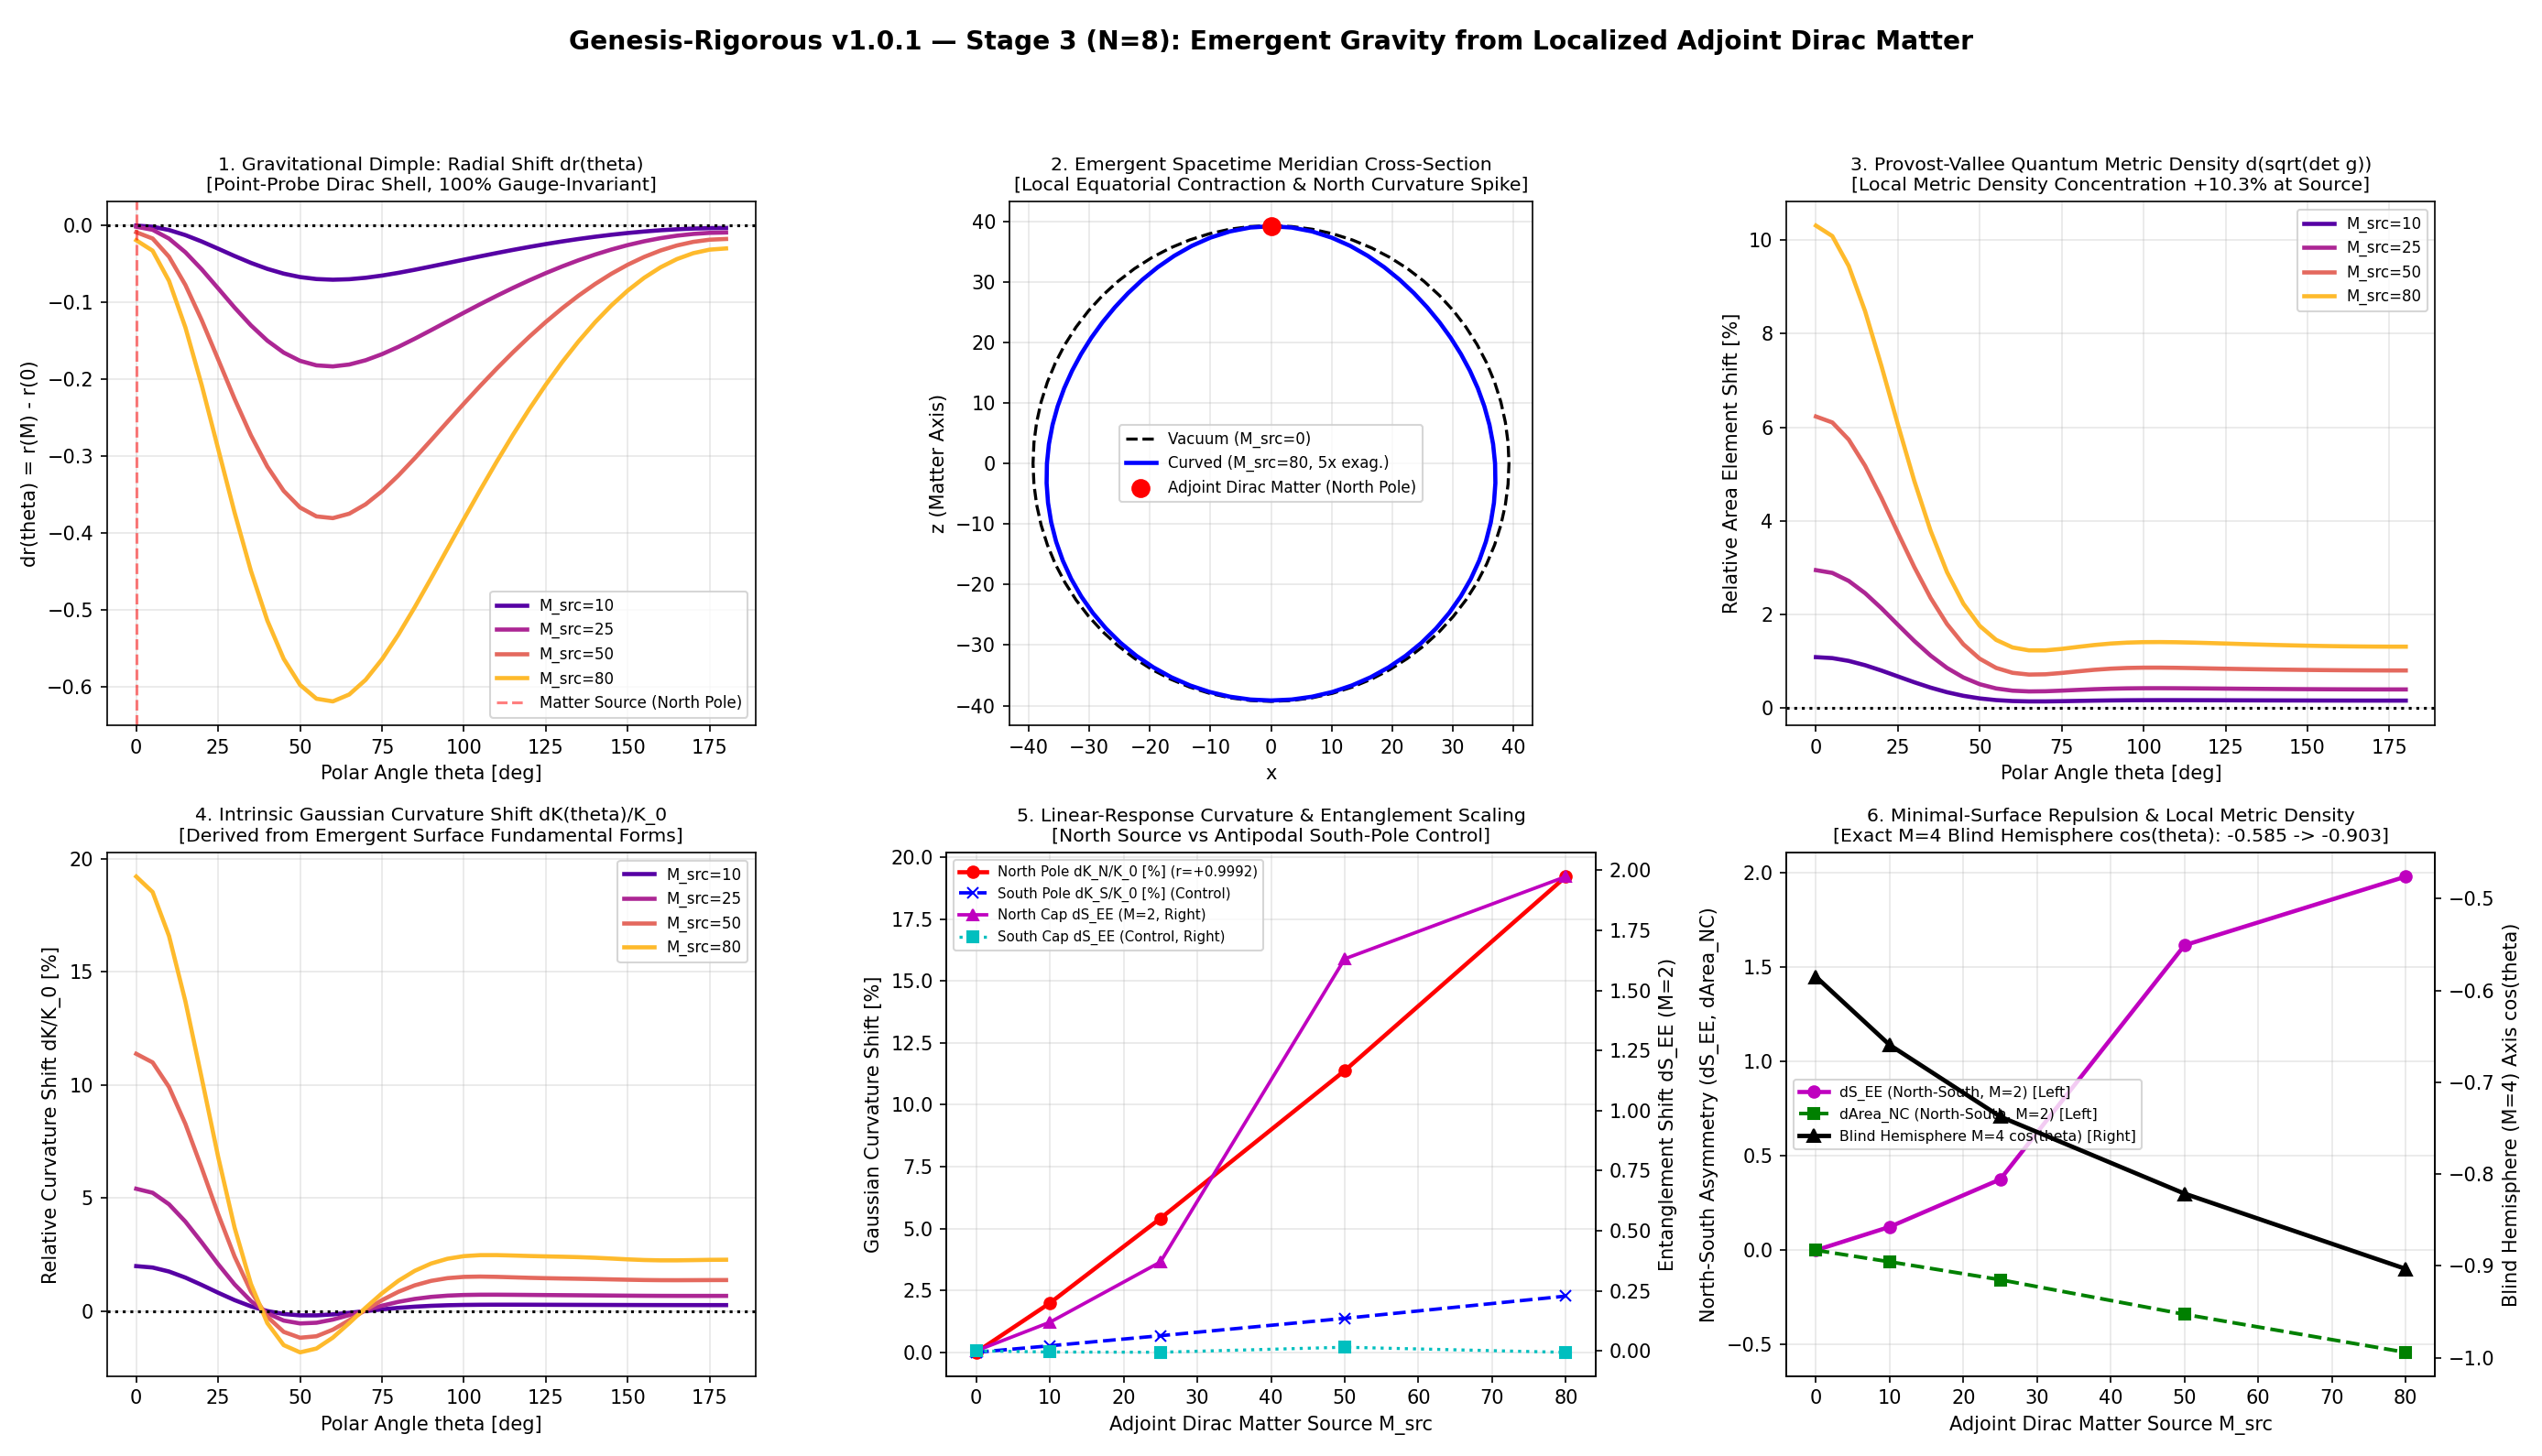
\includegraphics[width=0.95\textwidth]{figures/fig3_stage3_gravity_N8.png}
  \caption{Inherited \texttt{v1.0.1} single-body Dirac elastic membrane sweep at $N=8$ (embedded ``Emergent Gravity'' title superseded by Experiment~3).}
  \label{fig:stage3}
\end{figure}

\begin{figure}[H]
  \centering
  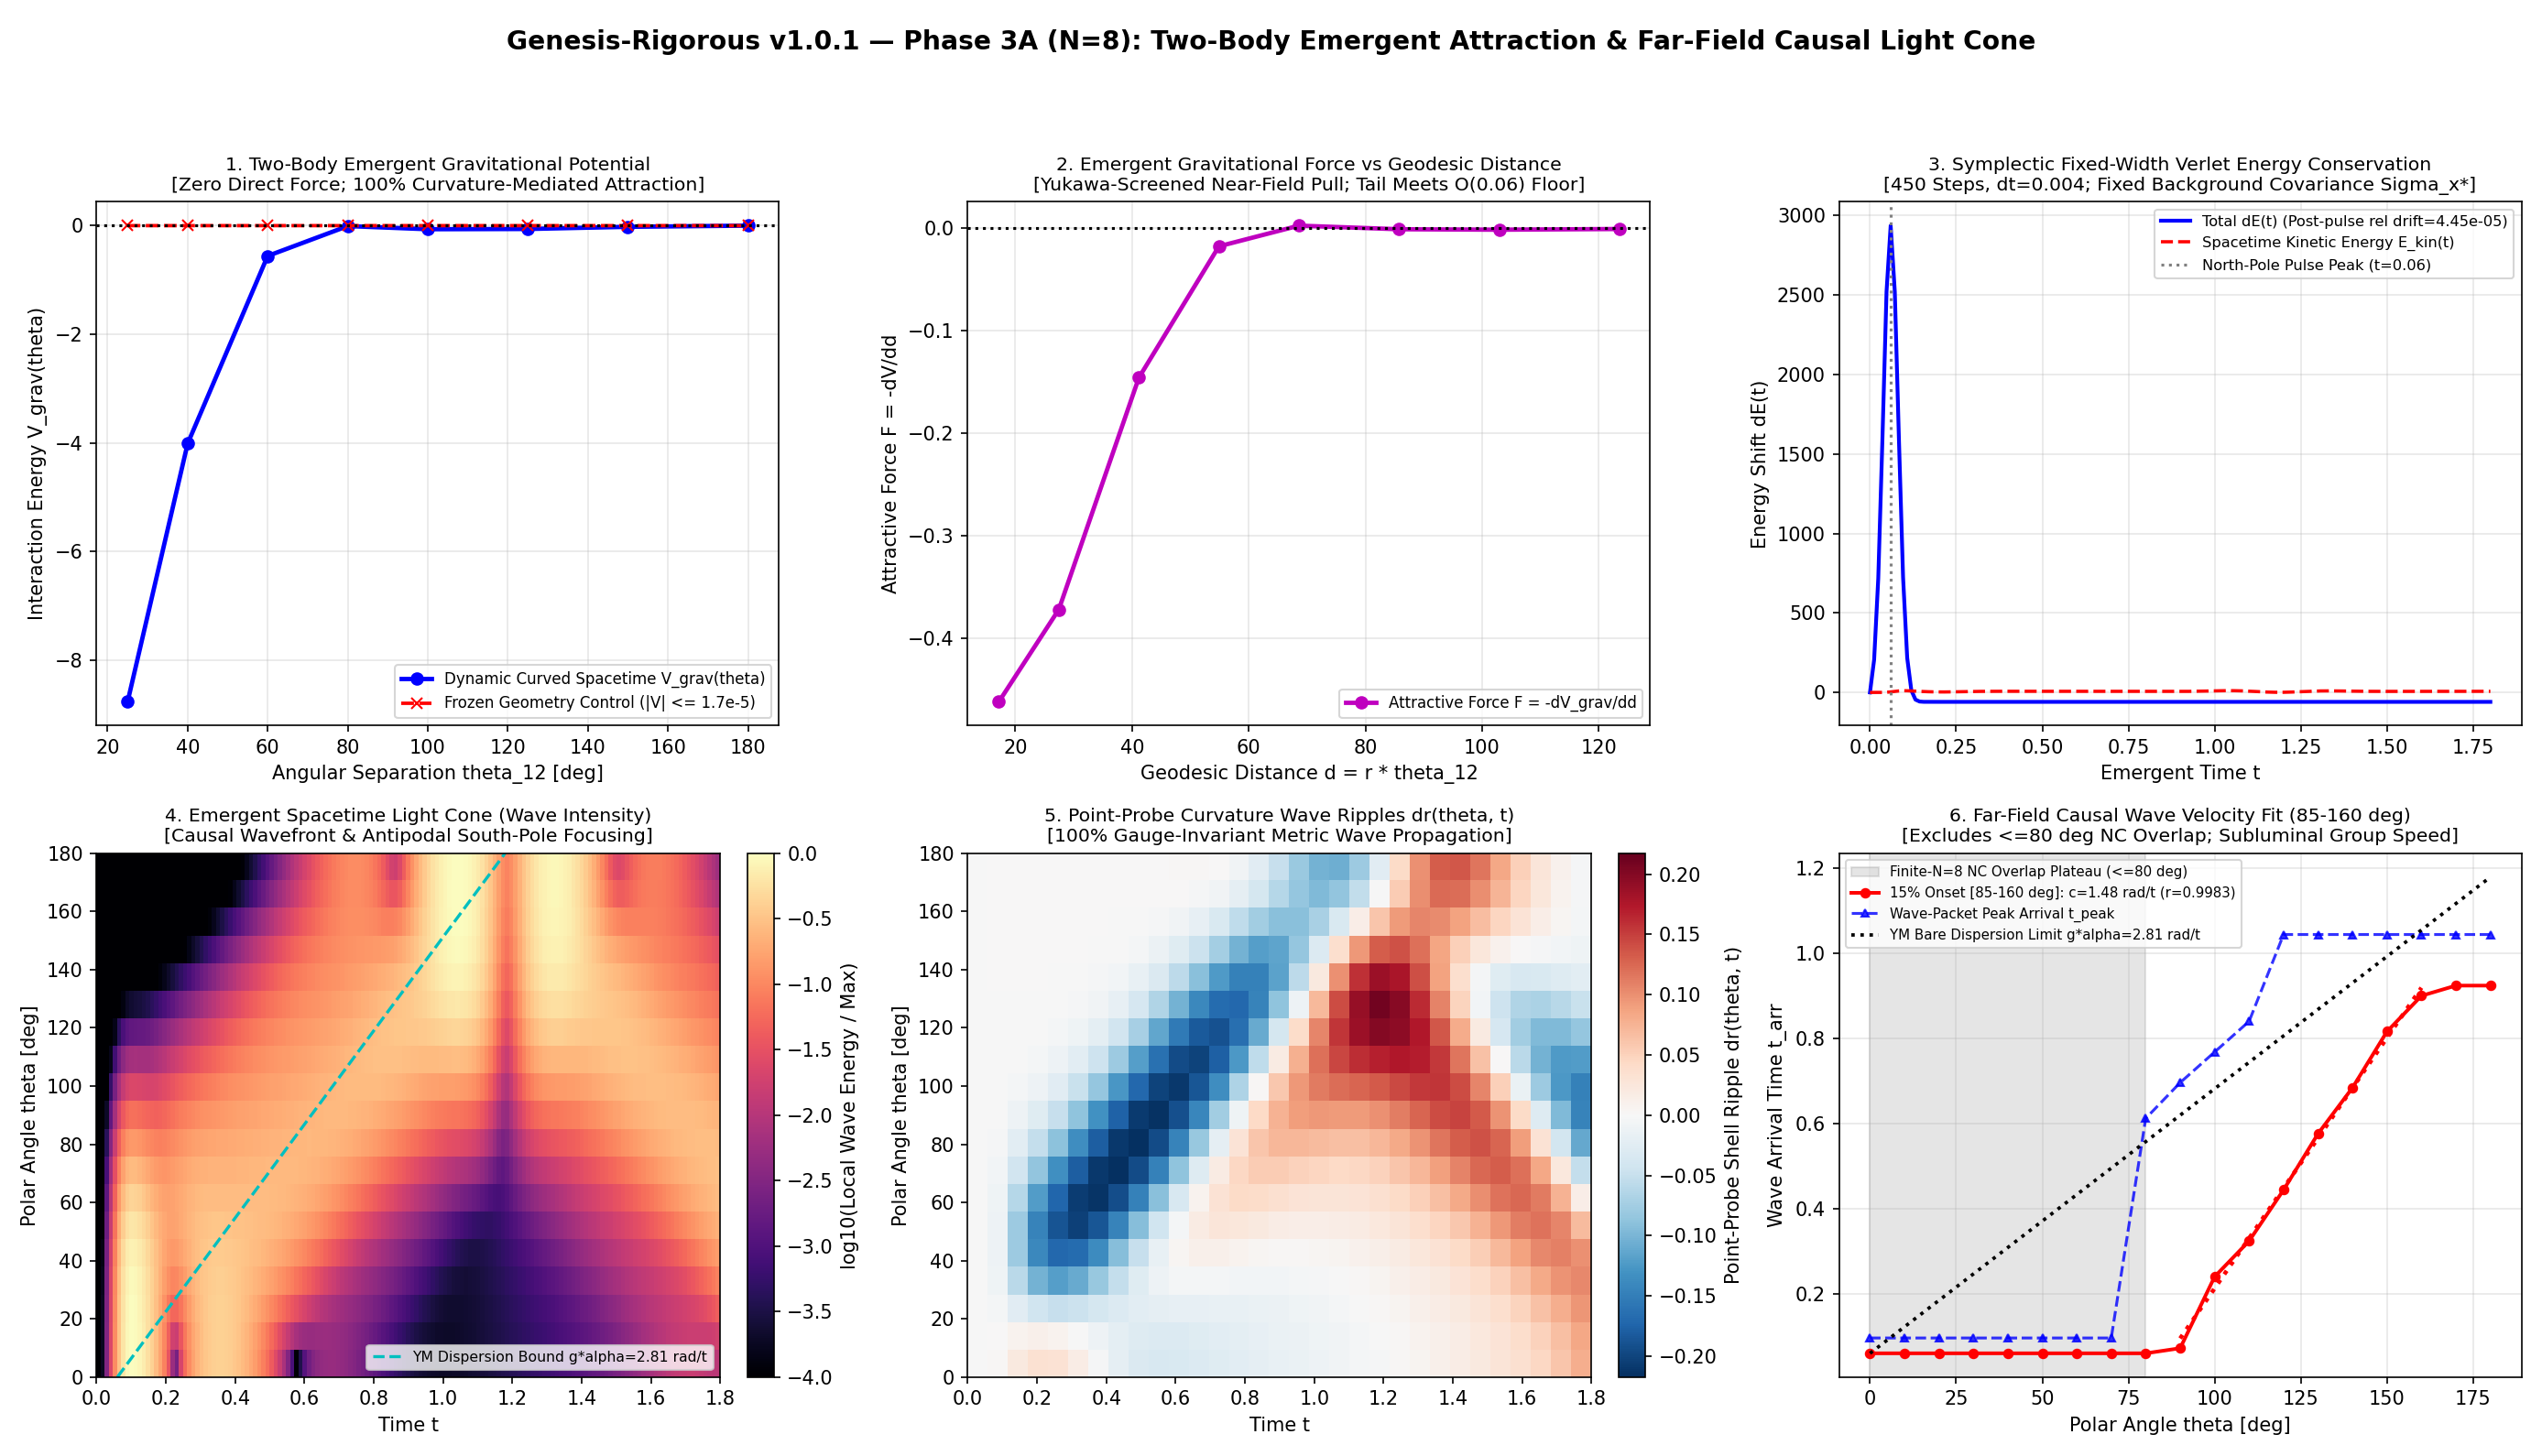
\includegraphics[width=0.95\textwidth]{figures/fig4_phase3a_dynamics.png}
  \caption{Inherited \texttt{v1.0.1} two-packet interaction and fixed-width symplectic dispersive wave dashboard at $N=8$ (embedded ``light cone'' header interpreted as dispersive elastic wave propagation).}
  \label{fig:phase3a}
\end{figure}

\begin{figure}[H]
  \centering
  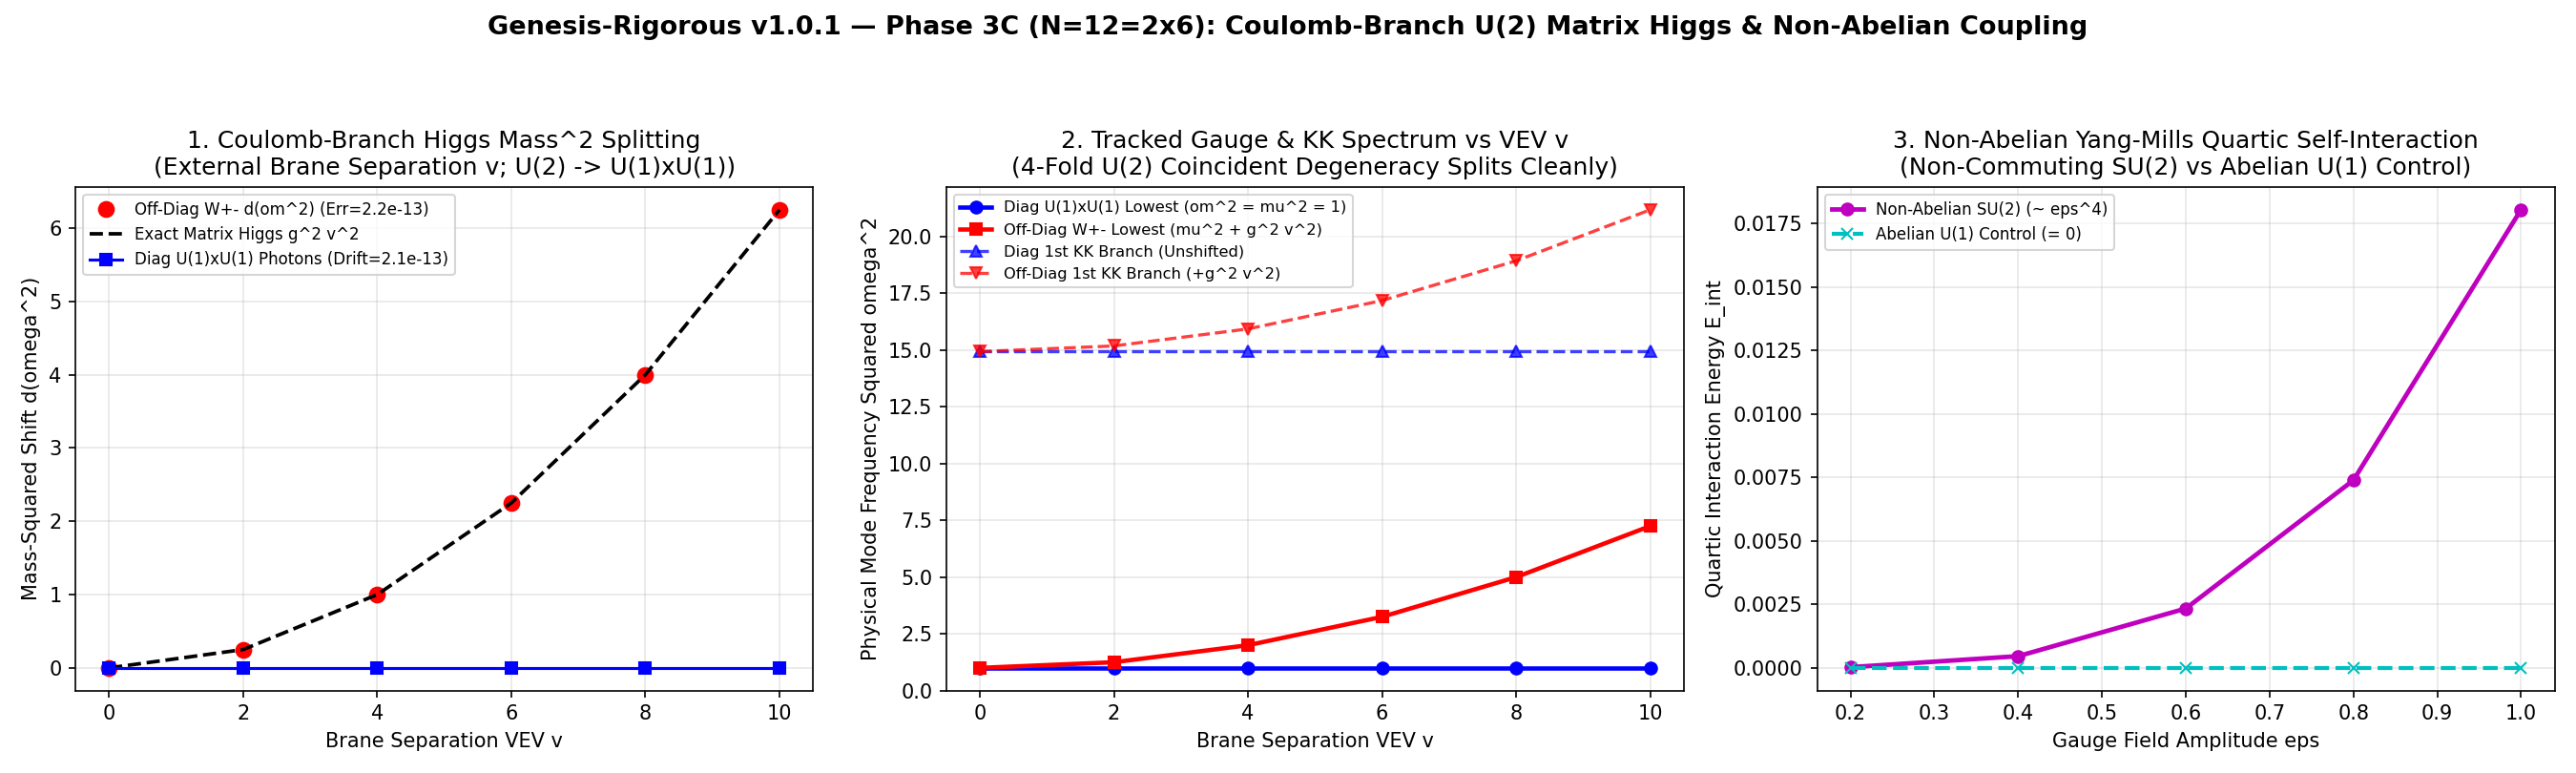
\includegraphics[width=0.95\textwidth]{figures/fig6_phase3c_gauge_higgs.png}
  \caption{Inherited \texttt{v1.0.1} $U(2)$ Coulomb-branch Higgs algebraic identity verification ($N=12=2\times 6, D=4$).}
  \label{fig:phase3c}
\end{figure}

\begin{figure}[H]
  \centering
  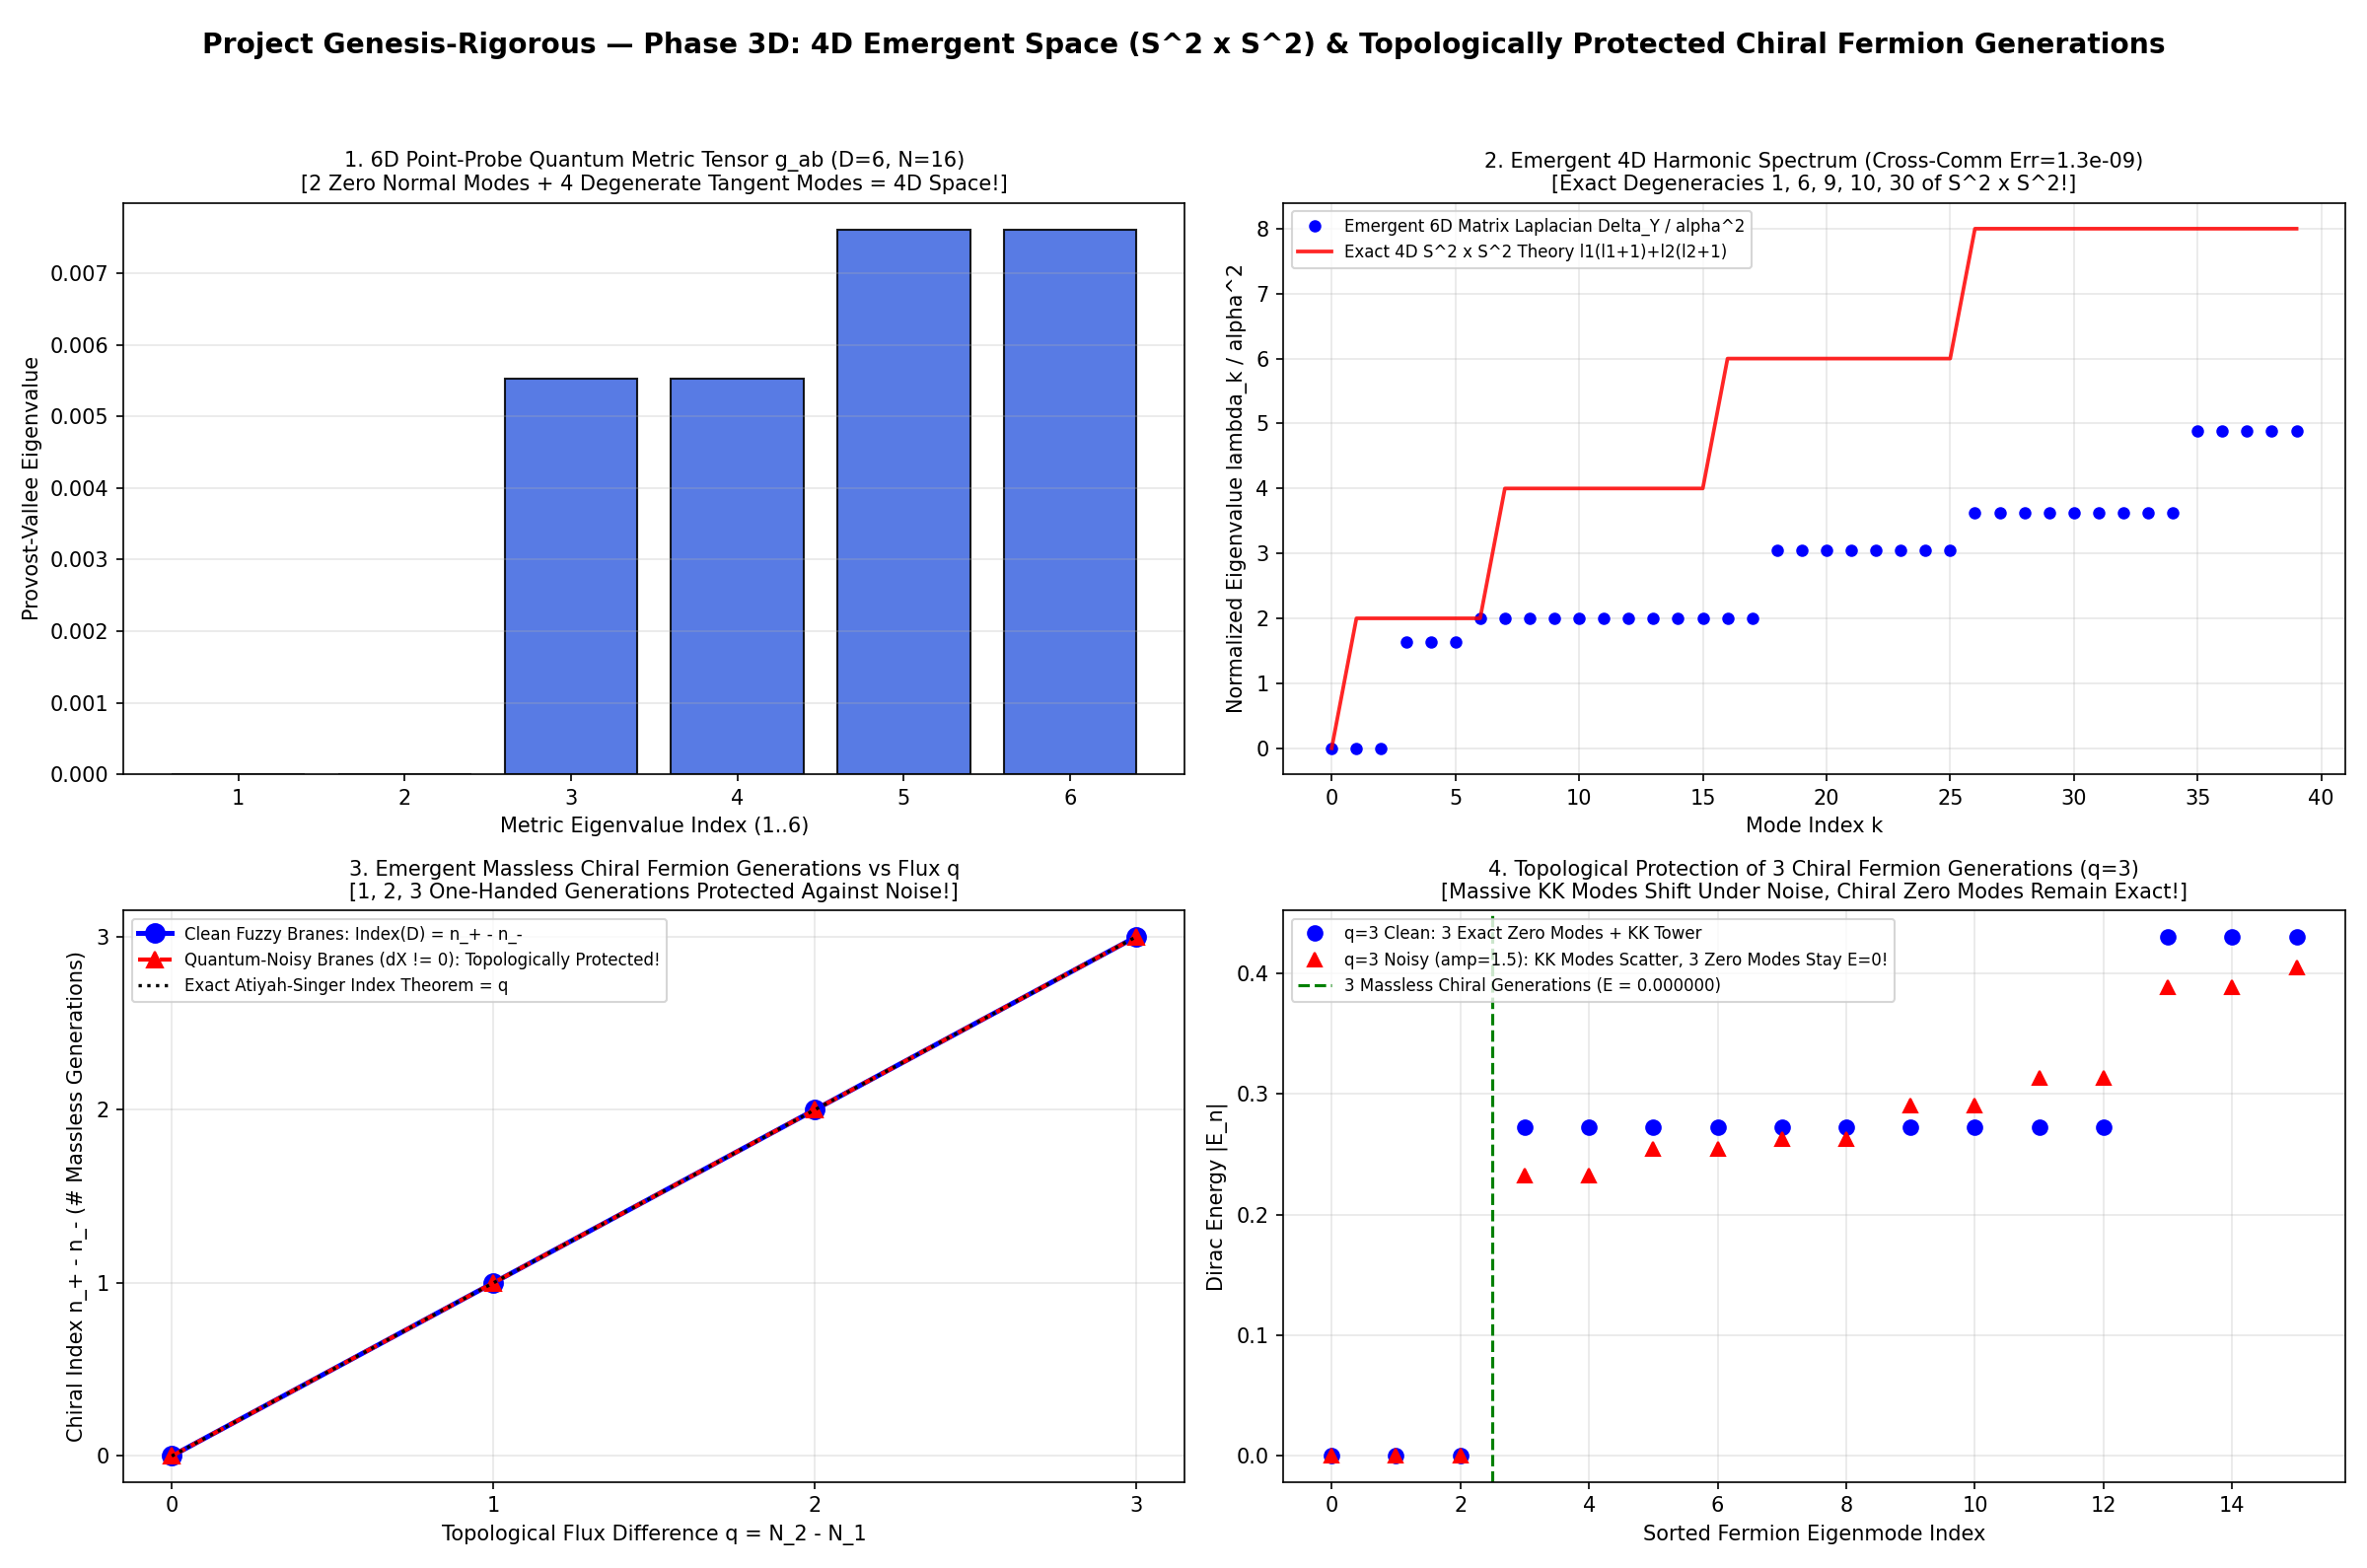
\includegraphics[width=0.95\textwidth]{figures/fig7_phase3d_4d_chiral.png}
  \caption{Inherited \texttt{v1.0.1} ultra-coarse 6D product representation ($3\times 4$ states) and fuzzy Ginsparg--Wilson monopole zero-mode index verification ($q=0,1,2,3$).}
  \label{fig:phase3d}
\end{figure}

% ==============================================================================
\section{Discussion, Remaining Limitations, and Outlook}
\label{sec:discussion}
% ==============================================================================

By closing the three concrete methodological holes of \texttt{v1.0.1} with actual code and new benchmark data, \texttt{Genesis-Rigorous v1.0.2} establishes a transparent, reproducible PC-scale framework for exploring emergent fuzzy-sphere geometry and subregion quantum entanglement in matrix quantum mechanics. Four honest limitations remain well-defined targets for future work:
\begin{enumerate}
  \item \textbf{Lattice continuum extrapolation and larger-$N$ HMC:} Experiment~2 ran exact gauged HMC at $N=4, L=12, \beta=3.0$ ($a=0.25$), where finite-$a$ UV dispersion accounts for $+15.74$ of the $+18.45$ energy offset on stiff spheres. Extrapolating $a \to 0$ ($L=16, 24, 32$) and scaling HMC to $N=6, 8, 12$ will allow direct continuum thermodynamic-limit fits of $\nu_c^{\mathrm{quantum}}(g, N)$ and the confinement transition.
  \item \textbf{Gauge-singlet subregion entanglement:} While Experiment~1 establishes decisive $O(N)$ vs.\ $O(N^2)$ scaling separation in both traceless $S_{\mathrm{TN}}^{\mathfrak{su}(N)}$ and Gaussian HFB $S_{\mathrm{bos}}$, $S_{\mathrm{bos}}$ is still computed on non-singlet HFB wave-packets regulated by $\omega_{\min}=0.15$. Measuring entanglement directly on gauge-singlet neural VMC states~\cite{Han2020} or replica-trick HMC ensembles remains an important next step.
  \item \textbf{Myers $SO(3)$ Hamiltonian structure:} The core \texttt{v1.0.2} Hamiltonian retains the explicit $SO(3)$-symmetric Myers flux term. Removing this symmetry bias to map emergent manifolds across generic random noncommutative matrix Hamiltonians (and bounding strongly coupled matrix ground states via semidefinite Matrix Bootstrap) is being pursued separately as an independent research branch.
  \item \textbf{Physical scope relative to $(3+1)$D quantum gravity:} As established by Experiment~3, $(0+1)$D bosonic three-matrix fuzzy spheres exhibit noncommutative elastic shell mechanics rather than massless $(3+1)$-dimensional spin-2 Einstein gravity or Standard Model flavor hierarchies.
\end{enumerate}

% ==============================================================================
\section{Software Availability and Reproducibility}
\label{sec:repro}
% ==============================================================================

\texttt{Genesis-Rigorous v1.0.2} is released under the MIT License (extending archived \texttt{v1.0.1}, Zenodo DOI \href{https://doi.org/10.5281/zenodo.24537568}{\texttt{10.5281/zenodo.24537568}}). All 20 unit tests and all three new \texttt{v1.0.2} experiments execute directly via the unified CLI on any standard PyTorch desktop:
\begin{verbatim}
python -m unittest discover -s tests -v    # 20-test verification suite (~3.6 s)
python genesis_cli.py entanglement-scaling # Exp 1: Traceless su(N) & HFB N-scaling (~45 s)
python genesis_cli.py phase-hmc            # Exp 2: nu-transition & HMC vs HFB melting (~6 min)
python genesis_cli.py membrane-control     # Exp 3: Dirac vs Tr(rho Y^2) control (~3.5 min)
\end{verbatim}
All six inherited \texttt{v1.0.1} subcommands (\texttt{phase1}, \texttt{gravity}, \texttt{realtime}, \texttt{large-n}, \texttt{gauge}, \texttt{chiral}) remain fully functional and backward-compatible.

% ==============================================================================
\section*{Acknowledgments and AI Collaboration Statement}
% ==============================================================================

This software testbed and manuscript were developed through an interactive human--AI collaboration between the human author (Alpha496) and Google Gemini (within the Antigravity development environment), which assisted with mathematical derivations, PyTorch/CUDA implementation (including the traceless $\mathfrak{su}(N)$ BdG projection and exact gauged lattice HMC engine), automated unit-test design, and manuscript drafting. Crucially, to break single-agent closed-loop blind spots, the preceding \texttt{v1.0.1} manuscript underwent an independent adversarial review by an external AI reviewer (Claude Opus), whose sharp mathematical critique directly motivated all three new \texttt{v1.0.2} code upgrades, the exact Schwinger--Dyson/HMC benchmarks, and the honest scope corrections reported here. The human author conceived the research direction, decided all experimental priorities, executed and verified all simulations on local hardware, and assumes full responsibility for all scientific claims and released code.

\bibliographystyle{unsrt}
\bibliography{references}

\end{document}
